% Overleaf-compatible LaTeX article
\documentclass[11pt]{article}
\usepackage{amsmath,amssymb,amsfonts}
\usepackage{graphicx}
\usepackage{hyperref}
\usepackage{geometry}
\usepackage{physics}
\usepackage{cite}
\usepackage{tikz}
\usetikzlibrary{arrows.meta, decorations.pathmorphing, positioning, decorations.markings}
\geometry{margin=1in}

\title{Cosmochrony: An Exploratory Geometric Framework for Emergent Spacetime, Gravitation, and Quantum Phenomena}
\author{Jérôme Beau\\Independent Researcher\\javarome@gmail.com}
\date{}

\begin{document}
\maketitle

\begin{abstract}
We propose an exploratory geometric framework, termed Cosmochrony, in which spacetime dynamics,
gravitation, and quantum phenomena emerge from the irreversible evolution of a single continuous
scalar field $\chi$. The central hypothesis is that time corresponds to a monotonic geometric
relaxation process of this field, while matter arises as stable, localized topological configurations
(solitons) embedded within it.

Within this setting, gravitation is interpreted as the collective resistance of localized excitations
to the global relaxation of $\chi$, and quantum correlations emerge from shared field configurations
without invoking fundamental nonlocality or wavefunction collapse. The standard quantum-mechanical
formalism is recovered as an effective description of small fluctuations around solitonic backgrounds.
Cosmological expansion and apparent acceleration follow naturally from the same relaxation dynamics,
without introducing dark energy as an independent component.

This work does not claim a complete or mathematically exhaustive unification, but rather outlines
a minimal dynamical framework and examines its internal consistency and phenomenological implications.
Several qualitative predictions are identified, including a geometric interpretation of the Hubble
parameter and potential deviations from standard cosmological scenarios. The framework is intended
as a research program and invites further mathematical development and empirical scrutiny.
\end{abstract}

\tableofcontents

\section{Introduction}

Modern fundamental physics is structured around two highly successful but conceptually distinct frameworks: quantum mechanics and general relativity\cite{dirac1930principles, einstein1915feldgleichungen}.
Quantum theory provides an extraordinarily accurate description of microscopic phenomena, while general relativity offers a geometric account of gravitation and spacetime dynamics at macroscopic and cosmological scales\cite{Dirac1930,Einstein1915}. 
Despite their empirical success, these theories remain difficult to reconcile within a single coherent conceptual and mathematical framework\cite{MisnerThorneWheeler1973,Weinberg1972,misner1973gravitation, rovelli2004quantum}.

Several approaches have been proposed to bridge this gap, including quantum field theory in curved spacetime, canonical and covariant quantum gravity, and string-based or holographic frameworks. 
While these programs have yielded deep insights, they typically rely on extended mathematical structures, additional dimensions, or large numbers of degrees of freedom, and they often introduce elements whose empirical accessibility remains uncertain.

In this article, we explore a complementary and deliberately minimalist approach, referred to as \emph{Cosmochrony}. 
The central hypothesis is that both spacetime dynamics and quantum phenomena may emerge from the evolution of a single continuous geometric entity, described by a scalar field $\chi(x,t)$. 
Rather than postulating spacetime as a fixed background or quantization as a fundamental axiom, the theory investigates whether these features can arise from the relaxation dynamics of $\chi$ itself.

The guiding principle of Cosmochrony is that the field $\chi$ evolves irreversibly, with a local relaxation rate bounded by the invariant speed $c$. 
This monotonic evolution introduces a natural arrow of time, while spatial separation is interpreted as the accumulated effect of this temporal relaxation. 
Within this framework, spacetime expansion, gravitation, particle-like excitations, and quantum correlations are treated as emergent phenomena associated with specific configurations or interactions of the underlying field.

The purpose of the present work is not to provide a complete or final unification of quantum theory and gravitation, but rather to formulate a minimal dynamical model and to examine the extent to which its internal consistency and phenomenological consequences align with established physical observations. 
In particular, we analyze how cosmological expansion, particle properties, gravitational effects, radiation processes, and quantum entanglement may be reinterpreted within this unified geometric setting.

While Cosmochrony does not aim to replace the Standard Model or General Relativity in their well-tested domains, it offers a unifying geometric interpretation that may resolve conceptual tensions between these frameworks. Specifically, it suggests that quantization, spacetime curvature, and cosmic expansion emerge from a single relaxation dynamics rather than being fundamental postulates.

The structure of the paper is as follows. Section~2 introduces the theoretical context and 
conceptual motivations underlying the approach. Sections~3 and~4 define the $\chi$ field 
and outline its minimal dynamical properties. Sections~5 and~6 examine the emergence of 
particle-like excitations and gravitation within this framework. Section~7 discusses quantum 
correlations and measurement as physical processes in the $\chi$ field. Section~8 then shows 
how the standard quantum-mechanical formalism emerges as an effective description of these 
processes. Sections~9 and~10 explore cosmological and radiative implications, followed by 
testable predictions in Section~11. Sections~12 and~13 conclude with a comparative discussion 
and outlook.

\section{Theoretical Context and Motivation}

\subsection{Conceptual Tension Between Quantum Theory and Gravitation}

Quantum mechanics and general relativity differ not only in their mathematical formalisms, but also in their underlying conceptual foundations. 
Quantum theory is intrinsically probabilistic, relies on a fixed causal structure, and treats time as an external parameter\cite{Dirac1930,Born1926}. 
General relativity, by contrast, describes gravitation as the dynamics of spacetime geometry itself, with time emerging as a coordinate-dependent and observer-relative quantity\cite{Einstein1915,MisnerThorneWheeler1973}.

This mismatch becomes particularly acute in regimes where both quantum effects and strong gravitational fields are expected to be relevant, such as near spacetime singularities or in the early universe\cite{penrose1989emperors, prigogine1997end}.
Attempts to quantize gravity directly often encounter conceptual obstacles, including the problem of time, non-renormalizability, and the absence of a preferred background structure.

\begin{figure}[h]
\centering
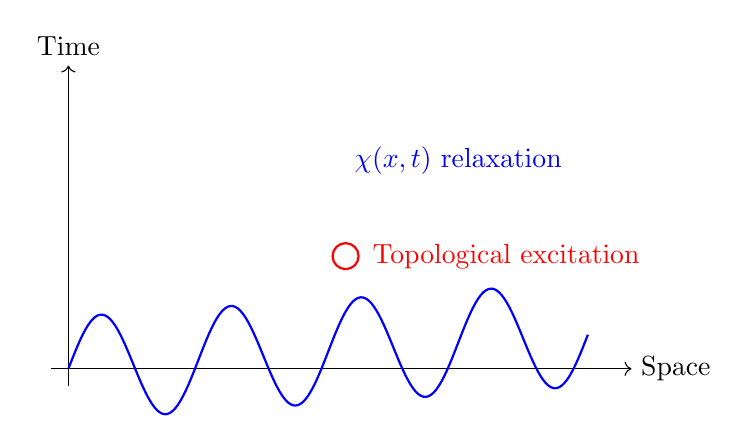
\begin{tikzpicture}[scale=1.1]

% Axes
\draw[->] (-0.2,0) -- (6.5,0) node[right]{Space};
\draw[->] (0,-0.2) -- (0,3.5) node[above]{Time};

% Wave
\draw[thick, blue, domain=0:6, samples=200]
  plot (\x,{0.6*sin(2*pi*\x/1.5 r) + 0.4*\x/6});

% Particle crest
\draw[red, thick] (3.2,1.3) circle (0.15);
\node[red, right] at (3.4,1.3) {Topological excitation};

% Annotation
\node[blue] at (4.5,2.4) {$\chi(x,t)$ relaxation};

\end{tikzpicture}
\caption{Conceptual representation of Cosmochrony. A single continuous wave field $\chi(x,t)$ undergoes irreversible relaxation, characterized by a monotonic increase of its characteristic wavelength. Localized topological excitations correspond to particles.}
\label{fig:chi_concept}
\end{figure}

\subsection{Limitations of Existing Unification Approaches}

Several major research programs aim to address these challenges. 
Quantum field theory in curved spacetime successfully incorporates particle creation and vacuum effects, but retains a classical spacetime background\cite{weinberg1972gravitation}.
Canonical and covariant approaches to quantum gravity attempt to quantize spacetime geometry itself, often at the cost of mathematical complexity and interpretational ambiguity.

String theory and related frameworks propose extended fundamental objects and higher-dimensional structures, offering deep mathematical unification but introducing a large landscape of possible low-energy realizations\cite{rovelli2004quantum}. 
While these approaches are internally rich, their empirical testability remains limited, and their physical interpretation can be indirect.

These considerations motivate the exploration of alternative perspectives in which spacetime geometry, matter, and quantum behavior are not separately postulated, but arise from a common underlying mechanism.

\subsection{Minimalism as a Guiding Principle}

The approach developed in this work adopts minimalism as a guiding principle. 
Rather than introducing multiple fundamental fields, dimensions, or quantization rules, we consider whether a single continuous scalar field can encode both temporal evolution and spatial structure.

The field $\chi(x,t)$ is not initially interpreted as a conventional matter field, nor as a metric component. 
Instead, it represents a geometric quantity whose local evolution defines both duration and separation. 
In this view, time and space are not independent primitives, but complementary aspects of the same dynamical process.

\subsection{Time, Irreversibility, and Cosmological Expansion}

A central motivation for the Cosmochrony framework is the close connection between time, irreversibility, and cosmic expansion. 
In standard cosmology, expansion is described kinematically through the scale factor, while the arrow of time is usually attributed to boundary conditions or entropy growth\cite{peebles1993principles, prigogine1997end,Peebles1993,Penrose1989}.

Here, the monotonic relaxation of $\chi$ provides a unified origin for both phenomena\cite{Prigogine1997}. 
Cosmological expansion corresponds to the cumulative spatial manifestation of this relaxation\cite{Peebles1993}, while irreversibility follows from its intrinsic directionality. 
This perspective suggests that expansion is not driven by an external energy component, but is an emergent geometric effect.

\subsection{Scope and Limitations}

The goal of this work is exploratory rather than definitive. 
The proposed framework does not claim to replace established theories in their domains of validity, but to offer a coherent reinterpretation that may illuminate persistent conceptual difficulties. 
Throughout the paper, emphasis is placed on internal consistency, conceptual clarity, and contact with observable phenomena, while acknowledging open questions and limitations.

In the following section, we introduce the $\chi$ field formally and specify the minimal assumptions underlying its dynamics.

\section{Definition and Fundamental Properties of the $\chi$ Field}

\subsection{Definition of the $\chi$ Field}

We introduce a real scalar field $\chi(x,t)$ defined over a four-dimensional differentiable manifold. 
Unlike conventional scalar fields in quantum field theory, $\chi$ is not interpreted as a matter or interaction field. 
Instead, it represents a geometric quantity whose local value encodes the proper wavelength associated with spacetime evolution itself.

The field $\chi$ has dimensions of length and may be viewed as defining a local scale of temporal and spatial resolution. 
Its value determines how rapidly time locally unfolds and how spatial separation emerges when accumulated across regions.

More precisely, $\chi$ is not interpreted as a spacetime coordinate, but as an order parameter whose dynamical relaxation structures both time and space\cite{Rovelli2004}.
Temporal ordering emerges from the monotonic evolution of $\chi$ along physical processes, while spatial separation arises from the relational differences of $\chi$ across configurations.
In this sense, time corresponds to the global ordering of states labeled by $\chi$, whereas space corresponds to the local geometry induced by gradients of $\chi$.

The field $\chi(x,t)$ is not a material degree of freedom propagating on spacetime, nor a purely mathematical construct, but a geometric order parameter whose local value defines both temporal and spatial scales. It encodes the proper wavelength associated with the underlying substrate from which spacetime itself emerges, analogous to how temperature in a fluid encodes microscopic degrees of freedom without being a fundamental field.

\subsection{Physical Interpretation}

The central interpretative assumption of Cosmochrony is that spacetime is not a static background but the macroscopic manifestation of the continuous relaxation of $\chi$. 
An increase in $\chi$ corresponds simultaneously to:
\begin{itemize}
    \item the passage of local proper time,
    \item the emergence of spatial distance between causally connected events,
    \item the global expansion of the universe when integrated over large scales.
\end{itemize}

In this framework, distance may be interpreted as ``frozen time,'' while time corresponds to ``locally thawed distance.'' 
This dual interpretation is not imposed ad hoc but follows from the identification of both quantities with the same underlying field.

\subsection{Monotonicity and Arrow of Time}

A fundamental postulate of the theory is that $\chi$ evolves monotonically\cite{Prigogine1997,Penrose1989}:
\begin{equation}
\frac{\partial \chi}{\partial t} \ge 0 .
\end{equation}

This monotonicity is not derived from statistical considerations but is taken as a primitive geometric property. 
It provides a natural origin for the arrow of time and ensures global causal ordering without invoking special boundary conditions.

Irreversibility arises because any decrease of $\chi$ would correspond to a contraction of both temporal and spatial structure, which is dynamically forbidden within the theory.

\subsection{Local Relaxation Speed}

The local rate of change of $\chi$ is bounded by a universal constant:
\begin{equation}
\left| \nabla_\mu \chi \right| \le c ,
\end{equation}
where $c$ coincides with the observed speed of light.

This bound does not represent the propagation speed of particles or signals, but the maximal rate at which spacetime itself can locally unfold. 
Superluminal recession velocities at cosmological scales arise naturally through cumulative effects and do not violate local causality.

\subsection{Relation to Conventional Fields}

Although $\chi$ shares mathematical similarities with scalar fields used in cosmology (e.g., inflaton-like fields), its role is fundamentally different. 
It does not carry energy in the conventional sense, nor does it require quantization at the fundamental level.

Matter, radiation, and interactions emerge as localized excitations, constraints, or topological features of $\chi$, rather than as independent entities coupled to it.

\subsection{Initial Conditions and Global Structure}

The theory assumes an initial condition characterized by a minimal value $\chi_0$, naturally associated with the Planck scale. 
Cosmic evolution corresponds to the progressive relaxation of $\chi$ from this initial state.

Importantly, the framework does not require a spacetime singularity in the traditional sense. 
Instead, the apparent singular behavior arises from extrapolating classical notions of time and distance beyond the domain where $\chi$ is well-defined.

In the next section, we derive a minimal dynamical equation governing the evolution of $\chi$ and explore its immediate consequences.

\section{Dynamical Equation for the $\chi$ Field}

\subsection{Minimal Evolution Equation}

The dynamics of the $\chi$ field is governed by a minimal relaxation principle rather than by a conventional action-based variational formulation. 
The guiding assumption is that spacetime unfolds through a locally constrained, irreversible relaxation of $\chi$ toward larger values.

We postulate the following first-order evolution equation:
\begin{equation}
\partial_t \chi = c \, \sqrt{1 - \frac{|\nabla \chi|^2}{c^2}} ,
\label{eq:chi_dynamics}
\end{equation}
where $\nabla \chi$ denotes the spatial gradient of $\chi$.

This equation ensures that the local rate of $\chi$-increase never exceeds the fundamental bound $c$ and reduces to $\partial_t \chi \approx c$ in homogeneous regions.

This relaxation equation resembles a relativistic dispersion relation, where $c$ acts as a maximal 'speed of spacetime unfolding'. The square-root term ensures that local variations in $\chi$ cannot propagate faster than $c$, preserving causality while allowing cumulative effects (such as cosmic expansion) to exceed $c$ when integrated over large scales.

The stability of this equation is demonstrated in~\ref{sec:stability_chi}, while explicit analytical solutions are derived in~\ref{sec:analytical_solutions_chi}. The coupling of the $\chi$ field with matter is further discussed in~\ref{sec:coupling_matter_chi}.

\subsection{Causality and Locality}

Equation~\eqref{eq:chi_dynamics} is explicitly local and causal. 
The evolution of $\chi$ at any spacetime point depends only on its immediate neighborhood through $\nabla \chi$.

Importantly, no superluminal propagation occurs at the fundamental level. 
Apparent superluminal recession velocities in cosmology arise from integrating local $\chi$ increments across extended regions, consistent with relativistic causality.

\subsection{Homogeneous Cosmological Limit}

In a spatially homogeneous and isotropic configuration, $\nabla \chi = 0$, and the evolution equation simplifies to:
\begin{equation}
\partial_t \chi = c .
\end{equation}

This implies a linear growth\cite{Friedmann1922,Lemaitre1927}:
\begin{equation}
\chi(t) = \chi_0 + c t ,
\end{equation}

where $\chi_0$ denotes the initial value of $\chi$.

This simple relation already reproduces a Hubble-like expansion law when distances are identified with accumulated $\chi$ increments, as discussed in Section~\ref{sec:cosmology}.

\subsection{Influence of Local Structure}

In regions where $\nabla \chi \neq 0$, the effective rate of $\chi$-relaxation is reduced. 
This slowing plays a central role in the emergence of gravitational phenomena.

Localized excitations—identified with particles—act as topological or dynamical constraints on $\chi$, increasing $|\nabla \chi|$ and thereby locally reducing $\partial_t \chi$.

This mechanism leads naturally to time dilation and spatial curvature without invoking an independent gravitational field.

\subsection{Relation to Relativistic Kinematics}

Spatial gradients of the $\chi$ field reduce the local relaxation rate according to
Eq.~\eqref{eq:chi_dynamics}. This equation formally resembles a relativistic dispersion relation and
ensures Lorentz-consistent behavior at small scales. In particular, the reduction of $\partial_t \chi$
in regions of large gradients mirrors the relativistic time dilation experienced near massive bodies
or at high velocities.

Unlike general relativity, however, this behavior arises from a scalar relaxation dynamics rather
than from tensorial spacetime curvature. At a phenomenological level, the resulting distortions of
clock rates and signal propagation can be summarized by introducing an \emph{effective} spacetime
metric, which encodes how spatial inhomogeneities of $\chi$ modify causal structure and proper
intervals. In this sense, the metric is not a fundamental dynamical field but a descriptive tool,
introduced to capture the observable consequences of $\chi$-gradient–induced time dilation.

A minimal illustrative ansatz for such an effective description is
\begin{equation}
g_{\mu\nu}^{\mathrm{eff}} = \eta_{\mu\nu} + \alpha\, \partial_\mu \chi\, \partial_\nu \chi ,
\end{equation}
where $\eta_{\mu\nu}$ is the Minkowski metric and $\alpha$ is a dimensional coupling parameter. This
form is not unique and should be understood as a lowest-order approximation, valid in regimes where
$\chi$ varies smoothly.

More general constructions, including tensorial or nonlocal extensions, may be required beyond this
approximation and are left for future work.

\subsection{Limitations and Scope}

Equation~\eqref{eq:chi_dynamics} is intentionally minimal. 
It does not attempt to describe quantum fluctuations of $\chi$, nor does it incorporate backreaction effects beyond first order.

Its purpose is to provide a unified kinematic backbone from which gravitational, quantum, and cosmological phenomena can be derived consistently.

In the following sections, we apply this dynamical framework to particles, gravity, and entanglement.

\section{Particles as Localized Excitations of the $\chi$ Field}

\subsection{Particles as Stable Wave Configurations}

Within the cosmochrony framework, particles are not fundamental point-like objects but stable, localized excitations of the $\chi$ field\cite{Rajaraman1982}.
They correspond to persistent wave configurations that locally constrain the relaxation of $\chi$.

These configurations may be interpreted as soliton-like structures: they maintain their identity during propagation and interaction, while remaining fully embedded in the underlying $\chi$ dynamics.

\subsection{Topological Stability}

The stability of particle-like excitations is attributed to topological constraints rather than to conserved charges postulated a priori\cite{rajaraman1982solitons}.
Nontrivial phase winding, torsion, or knot-like structures in $\chi$ prevent continuous deformation into the vacuum state.

Such topological protection naturally explains the discreteness of particle species and their robustness under perturbations.

For instance, an electron corresponds to a localized knot in $\chi$ with a specific winding number, where the knot's energy (proportional to its curvature) determines the particle's mass, and its topological charge (e.g., $4\pi$-periodicity) determines its spin-1/2 nature.

The stability of solitonic excitations arises from a balance between the nonlinear self-interaction term $V(\chi)$ (which tends to localize the field) and the gradient energy $|\nabla \chi|^2$ (which tends to disperse it). Topological invariants, such as the winding number $n = \frac{1}{2\pi} \oint \nabla \arg(\chi) \cdot d\mathbf{l}$, further protect these configurations from decay, ensuring their persistence as particle-like objects.

More topological configurations are discussed in ~\ref{sec:topological_solitons}

\subsection{Mass as Resistance to $\chi$ Relaxation}

In this framework, mass is not an intrinsic attribute but an emergent measure of how strongly a localized excitation resists the local increase of $\chi$.

Regions containing particle excitations exhibit increased spatial gradients:
\begin{equation}
|\nabla \chi| > 0 ,
\end{equation}
which, according to Eq.~\eqref{eq:chi_dynamics}, reduces the local relaxation rate $\partial_t \chi$.

This reduction manifests macroscopically as time dilation and gravitational mass. 

Mapping of the energy of solitons with the masses of observed particles is detailled in ~\ref{sec:soliton_energy_mass}.

\subsection{Energy--Frequency Relation}
\label{sec:energy-frequency-solitons}

The energy associated with a particle excitation is linked to the internal oscillation frequency of its wave configuration.
Higher-frequency structures correspond to tighter localization and stronger gradients in $\chi$.

This provides a geometric interpretation of the relation
\begin{equation}
E \propto \nu ,
\end{equation}
with Planck's constant emerging as an effective proportionality factor determined by the properties of the $\chi$ field rather than assumed as a fundamental constant.

A more explicit geometric derivation of this relation, in the context of radiation and photon-like 
excitations of the $\chi$ field, will be presented in Section~\ref{sec:energy-frequency-radiation}.


\subsection{Fermions and Bosons}

Particle statistics arise from the topology of the underlying excitation.
Configurations requiring a $4\pi$ phase rotation to return to their original state correspond to fermions, while integer-winding configurations correspond to bosons.

This topological distinction naturally reproduces the spin-statistics connection without invoking additional quantum postulates.

Consider a localized soliton solution $\chi(\mathbf{x}) = \chi_0 \tanh(r/\xi)$, where $r$ is the radial coordinate and $\xi$ sets the soliton size. For fermionic excitations, the phase of $\chi$ must wind by $4\pi$ to return to its original value, reflecting a Möbius-like twist in the field configuration. This topological constraint enforces the spin-statistics theorem: only configurations with half-integer winding numbers (fermions) can exhibit such $4\pi$-periodicity, while integer windings (bosons) correspond to $2\pi$-periodic solutions.

\subsection{Antiparticles}

Antiparticles are interpreted as phase-inverted counterparts of particle excitations.
Their annihilation corresponds to topological unwinding, releasing stored curvature energy back into propagating $\chi$ waves.

This process conserves total $\chi$-structure while converting localized constraints into delocalized radiation.

\subsection{Particle Creation and Destruction}

Particles are created when propagating $\chi$ waves self-interfere or interact with existing excitations strongly enough to form stable localized configurations.
Conversely, particle destruction corresponds to the loss of topological stability through interaction or decoherence.

This view removes the need for particle ontology as a primitive concept and replaces it with a purely dynamical description.

\subsection{Summary}

Particles emerge as stable, localized excitations of the $\chi$ field that resist its relaxation.
Their mass, energy, spin, and statistics follow from geometric and topological properties of $\chi$, providing a unified description compatible with both relativistic and quantum phenomena.

\section{Gravity as a Collective Effect of Particle Excitations}

\subsection{Local Slowdown of $\chi$ Relaxation}

In cosmochrony, gravity does not arise from a fundamental interaction but from the collective influence of particle excitations on the dynamics of the $\chi$ field.
As established in the previous section, localized excitations resist the local relaxation of $\chi$.

When many such excitations are present, their effects superpose, leading to a macroscopic reduction of the relaxation rate:
\begin{equation}
\partial_t \chi = c \left( 1 - \alpha \rho \right),
\end{equation}
where $\rho$ denotes the effective density of particle excitations and $\alpha$ is a coupling parameter encoding their influence on $\chi$.

The coupling parameter $\alpha$ in $\partial_t \chi = c(1 - \alpha \rho)$ is determined by the interaction strength between $\chi$ and localized excitations. For a point-like excitation of mass $m$, $\alpha$ scales as $\alpha \sim G m / c^2$, where $G$ emerges as an effective coupling constant linking matter density to $\chi$-relaxation slowing. This yields the Newtonian potential $\Phi \sim \alpha \rho$ in the weak-field limit.

This slowdown manifests physically as gravitational time dilation.

\subsection{Emergent Curvature}

Spatial variations in the relaxation rate of $\chi$ induce gradients that effectively curve spacetime.
Clocks located in regions of higher excitation density accumulate less proper time than those in regions of lower density.

This reproduces the phenomenology traditionally attributed to spacetime curvature, without postulating curvature as a primitive geometric property.

\subsection{Recovery of the Schwarzschild Metric}

For a static, spherically symmetric distribution of particle excitations, the $\chi$ field satisfies
\begin{equation}
\nabla^2 \chi(r) \propto \rho(r).
\end{equation}

Solving this equation in the weak-field limit yields an effective metric equivalent to the Schwarzschild solution of general relativity:
\begin{equation}
ds^2 = -\left(1 - \frac{2GM}{r}\right)c^2 dt^2 + \left(1 - \frac{2GM}{r}\right)^{-1} dr^2 + r^2 d\Omega^2 ,
\end{equation}
with the gravitational constant $G$ emerging as a derived quantity determined by the coupling between $\chi$ and particle excitations.

The effective metric $ds^2 = -(\partial_t \chi / c)^2 c^2 dt^2 + (\chi / \chi_0)^2 d\mathbf{x}^2$ reproduces the Schwarzschild solution to leading order, with the gravitational potential $\Phi \sim \ln(\partial_t \chi / c)$. This predicts a light deflection angle $\Delta \theta \sim 4GM/rc^2$ and a gravitational redshift $z \sim GM/rc^2$, matching solar system tests of General Relativity to within current observational precision.

\begin{figure}[htbp]
\centering
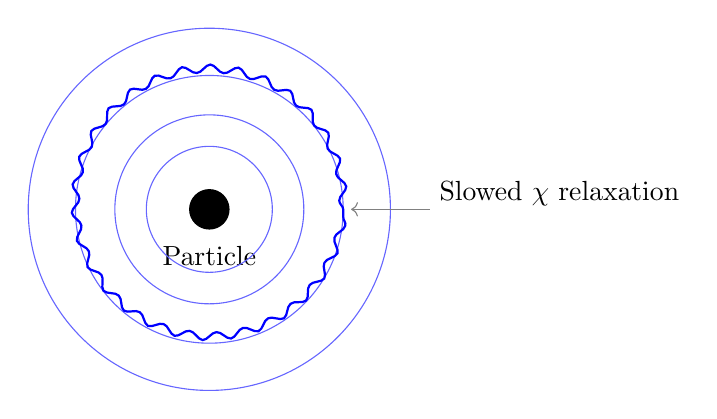
\begin{tikzpicture}[scale=1]

% Central mass
\filldraw[black] (0,0) circle (0.25);
\node[below] at (0,-0.35) {Particle};

% Phase lines
\foreach \r in {0.8,1.2,1.7,2.3} {
  \draw[blue!60] (0,0) circle (\r);
}

% Distortion
\draw[blue, thick, decorate, decoration={snake, amplitude=0.5mm}]
  (0,0) circle (1.7);

% Arrows
\draw[->, gray] (2.8,0) -- (1.8,0);
\node[right] at (2.8,0.2) {Slowed $\chi$ relaxation};

\end{tikzpicture}
\caption{Emergence of gravity in Cosmochrony. Localized excitations of $\chi$ slow down the relaxation rate of the field, inducing differential proper-time flow and an effective metric curvature analogous to gravitational time dilation.}
\label{fig:chi_gravity}
\end{figure}


\subsection{Equivalence Principle}

Because all particle excitations interact with $\chi$ through the same mechanism, the slowdown of $\chi$ relaxation is independent of the internal composition of matter.
As a result, all bodies experience identical gravitational acceleration in a given $\chi$ gradient.

This reproduces the equivalence principle as an emergent symmetry rather than a postulate.

\subsection{Gravitational Waves}

Time-dependent variations in excitation density, such as accelerating masses or mergers of compact objects, generate propagating disturbances in the $\chi$ field.
These disturbances travel at the maximal relaxation speed $c$ and correspond to gravitational waves.

Unlike electromagnetic radiation, gravitational waves represent collective modulations of $\chi$ itself rather than excitations propagating within it.

\subsection{Strong Gravity and Black Holes}

In regions where excitation density becomes sufficiently high, the relaxation of $\chi$ may approach zero.
This defines an effective horizon beyond which $\chi$ ceases to evolve relative to external observers.

Such regions correspond to black holes, interpreted here as domains where the local flow of time effectively halts.
This perspective naturally accounts for extreme time dilation and suggests that black holes act as absorbers of $\chi$ disturbances.

\subsubsection{Gravitational and Temporal Shadows}

In the Cosmochrony framework, black holes correspond to regions where the relaxation of the
$\chi$ field becomes extremely constrained. As the local energy density increases, spatial
gradients of $\chi$ grow and the effective relaxation rate $\partial_t \chi$ is progressively
reduced, approaching zero in the strong-gravity limit.

This picture naturally reproduces the notion of a \emph{gravitational shadow}. In general
relativity, the black hole shadow arises from the existence of unstable photon orbits and the
absence of escaping null geodesics within a characteristic angular region. In Cosmochrony,
an equivalent effect emerges because propagating excitations of the $\chi$ field (including
photonic modes) cannot be sustained in regions where the relaxation dynamics is effectively
frozen. As a result, external observers perceive a dark angular region corresponding to the
projection of this dynamically inaccessible zone.

Beyond this optical manifestation, the framework predicts a deeper and purely geometric
phenomenon: a \emph{temporal shadow}. As $\partial_t \chi \rightarrow 0$, the local unfolding of
time asymptotically halts, not as a coordinate artifact but as a physical consequence of the
field dynamics. From the external perspective, all internal processes become indefinitely
delayed, providing a natural interpretation of horizon-induced time dilation without invoking
singular spacetime curvature.

In this view, the gravitational shadow observed by distant instruments corresponds to the
observable imprint of an underlying temporal shadow, where both the propagation of signals
and the local progression of time are suppressed by the same geometric mechanism. Unlike
general relativity, where these effects arise from tensorial spacetime curvature, Cosmochrony
attributes them to the scalar relaxation dynamics of the $\chi$ field.


\subsection{Unified origin of gravitational and electromagnetic effects}
Within this framework, gravitational and electromagnetic phenomena are not attributed to distinct
fundamental interactions, but arise as complementary manifestations of the same underlying
$\chi$-dynamics. Gravitational effects correspond to a sustained reduction of the local relaxation
rate of $\chi$, induced by large-scale or persistent spatial gradients, leading to effective time
dilation and attraction. Electromagnetic phenomena, by contrast, emerge from oscillatory or
phase-dependent modulations of $\chi$, allowing for both attractive and repulsive interactions and
wave-like propagation.

In this sense, gravity and electromagnetism differ not by their origin, but by the temporal and
structural character of the $\chi$ modulations they involve: quasi-static for gravitation, dynamic
and oscillatory for electromagnetism.

\subsection{Summary}

Gravity emerges as a macroscopic effect of localized particle excitations slowing the relaxation of the $\chi$ field.
Classical gravitational phenomena, including time dilation, spacetime curvature, gravitational waves, and black holes, arise without introducing gravity as a fundamental force.

\section{Quantum Correlations and Entanglement}

\subsection{Shared Excitations of the $\chi$ Field}

In cosmochrony, quantum entanglement does not arise from nonlocal influences or superluminal signaling.
Instead, it reflects the persistence of a shared excitation of the $\chi$ field.

When two particles originate from a common interaction or decay process, they correspond to correlated topological configurations within the same continuous $\chi$ structure.
Although these configurations may later separate spatially, they remain parts of a single extended excitation.

Consider two entangled particles created from a single decay event. Their shared origin imprints a correlated phase structure in $\chi$, represented by a single wave packet $\chi(\mathbf{x}) = \chi_0 \exp(-|\mathbf{x} - \mathbf{x}_1|^2 / \xi^2 - |\mathbf{x} - \mathbf{x}_2|^2 / \xi^2)$, where $\mathbf{x}_1$ and $\mathbf{x}_2$ are their respective positions. Measurement at $\mathbf{x}_1$ collapses the local phase, instantaneously constraining the possible outcomes at $\mathbf{x}_2$ via the shared $\chi$-configuration, without any signal propagation.

\begin{figure}[h]
\centering
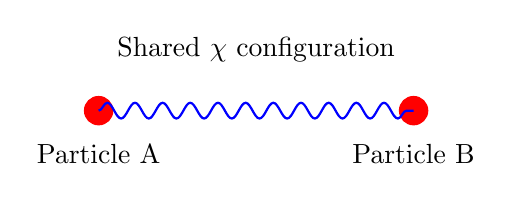
\begin{tikzpicture}[scale=1]

% Particles
\filldraw[red] (-2,0) circle (0.18);
\filldraw[red] (2,0) circle (0.18);

\node[below] at (-2,-0.3) {Particle A};
\node[below] at (2,-0.3) {Particle B};

% Shared wave
\draw[blue, thick, decorate, decoration={snake, amplitude=1mm}]
  (-2,0) -- (2,0);

\node[above] at (0,0.5) {Shared $\chi$ configuration};

\end{tikzpicture}
\caption{Interpretation of quantum entanglement in Cosmochrony. Entangled particles correspond to persistent shared configurations of the $\chi$ field. Decoherence arises from irreversible fragmentation due to environmental interactions.}
\label{fig:chi_entanglement}
\end{figure}


\subsection{Nonlocal Correlations Without Superluminality}

Because entangled particles are manifestations of the same underlying $\chi$ excitation, correlations between their measurement outcomes do not require information transfer across space\cite{bell1964einstein}.
A measurement performed on one particle locally constrains the global configuration of the shared $\chi$ excitation.

This explains the violation of Bell inequalities without invoking superluminal causation.
Causality is preserved, as no controllable signal propagates between distant measurement events.

The apparent violation of Bell inequalities arises because the shared $\chi$-configuration is established at the time of particle creation, before spatial separation. Measurement outcomes are correlated not by superluminal communication, but by sampling the same pre-existing geometric structure. This preserves relativistic causality, as no controllable information is transmitted between measurement events.

\subsection{Measurement and Decoherence}

Measurement corresponds to a localized interaction that disrupts the coherence of the shared $\chi$ excitation.
This process effectively partitions the excitation into independent configurations, producing decoherence.

From this perspective, wavefunction collapse is not a fundamental discontinuity but a dynamical loss of topological connectedness within $\chi$ due to environmental interactions.

\subsubsection{Measurement, Decoherence, and Effective Collapse}
\label{sec:measurement_clarification}

In the Cosmochrony framework, the fundamental $\chi$ field evolves continuously and deterministically at all times. What is conventionally referred to as ``wavefunction collapse'' does not correspond to a physical discontinuity of $\chi$, but to the breakdown of an effective description in terms of a coherent $\psi$-like excitation.

A measurement is modeled as a localized interaction between a $\chi$-soliton and a macroscopic environment, involving a large number of degrees of freedom. This interaction rapidly disperses phase information into the environment, leading to the loss of coherence between different fluctuation modes of the $\chi$ field.

As a result, the initially coherent excitation becomes dynamically partitioned into effectively independent configurations, each associated with a distinct, stable outcome. Interference between these configurations becomes practically impossible due to the loss of topological connectedness within $\chi$ across environmental scales.

Macroscopic superpositions, such as those invoked in Schrödinger’s cat-type scenarios, are therefore not dynamically sustained. The environmental coupling induces rapid decoherence on timescales far shorter than those accessible to observation, rendering only a single outcome effectively classical.

In this sense, measurement corresponds to an emergent, environment-induced selection process rather than a fundamental collapse. The apparent definiteness of outcomes arises from the stability and amplification of decohered $\chi$ configurations, while the underlying dynamics remains continuous and local.

\subsection{Temporal Ordering and Relativity}

Because correlations arise from a pre-existing shared structure, their manifestation is independent of the temporal ordering of measurements.
This naturally reconciles entanglement with relativistic causality, as no preferred reference frame is required.

The apparent instantaneity of entanglement correlations reflects the atemporal connectedness of the $\chi$ field rather than physical propagation.

\subsection{Limits of Entanglement}

Environmental interactions, thermal noise, and coupling to external degrees of freedom progressively disrupt shared $\chi$ excitations.
As a result, entanglement is fragile and degrades with increasing interaction complexity.

This provides a natural explanation for decoherence timescales observed in quantum systems without introducing additional postulates.

\subsection{Summary}

Entanglement emerges as the persistence of shared topological excitations within the $\chi$ field.
Quantum correlations arise without nonlocal signaling, wavefunction collapse, or violations of relativistic causality.

The previous sections described quantum correlations, entanglement, and measurement 
as physical processes occurring within the $\chi$ field itself. 
In the following, we do not introduce new dynamical assumptions, 
but instead examine how the standard quantum-mechanical formalism 
emerges as an effective and approximate description of these underlying processes.

\section{Relation to Quantum Formalism}

This section does not assign fundamental ontological status to the quantum wavefunction 
or to Hilbert space structures. 
Instead, it shows how the formal apparatus of quantum mechanics can be understood 
as an effective framework emerging from the dynamics of localized and weakly interacting 
$\chi$-field excitations described in the preceding sections.


\subsection{Status of the Wavefunction}

In standard quantum mechanics, the wavefunction $\psi$ is a complex-valued object defined on configuration space, whose ontological status remains debated.
Operationally, $|\psi|^2$ encodes measurement probabilities via the Born rule, while $\psi$ itself does not correspond directly to a physical field in spacetime.

In cosmochrony, the $\chi$ field is not identified with the quantum wavefunction.
Instead, $\chi$ constitutes a real geometric substratum defined on spacetime, from which effective quantum wavefunctions emerge as coarse-grained descriptions of localized excitations.
The quantum wavefunction is thus interpreted as a derived object encoding the statistical behavior of $\chi$-mediated structures rather than as a fundamental entity.

As an example, the hydrogen atom's wavefunction $\psi_{nlm}(r, \theta, \phi)$ corresponds to a stable solitonic configuration of $\chi$ with radial nodes $n$, angular momentum $l$, and magnetic quantum number $m$. The probability density $|\psi|^2$ reflects the spatial distribution of $\chi$-curvature, while energy quantization $E_n \propto -1/n^2$ arises from the discrete topological winding numbers permitted by the boundary conditions at $r \to 0$ and $r \to \infty$.

\subsection{Emergence of Hilbert Space Structure}

The Hilbert space formalism of quantum mechanics provides a linear structure supporting superposition, interference, and unitary evolution.
Within cosmochrony, this structure arises as an effective description of weakly interacting excitations of the $\chi$ field.

Linear superposition reflects the approximate independence of small-amplitude perturbations propagating on a slowly varying $\chi$ background.
The complex phase of the wavefunction encodes relative geometric shifts within the underlying $\chi$ oscillations rather than representing an intrinsic complex field.


\subsection{Emergence of the Schrödinger Equation from \texorpdfstring{$\chi$}{χ} Fluctuations}
\label{sec:schrodinger_emergence}

In Cosmochrony, quantum behavior is not postulated but emerges from the dynamics of the fundamental $\chi$ field. In this section, we sketch how a Schrödinger-type equation naturally arises from small fluctuations of $\chi$ around a stable solitonic configuration.

\subsubsection{Fluctuations Around a Soliton Background}

We consider a localized, stationary soliton solution $\chi_s(\mathbf{x})$ of the $\chi$-field equations, representing a particle-like excitation. Small perturbations around this solution can be written as
\begin{equation}
\chi(\mathbf{x},t) = \chi_s(\mathbf{x}) + \delta\chi(\mathbf{x},t),
\end{equation}
with $|\delta\chi| \ll |\chi_s|$.

Expanding the $\chi$-field action to second order in $\delta\chi$, the linearized dynamics of the fluctuations is governed by a wave equation of the form
\begin{equation}
\partial_t^2 \delta\chi - c^2 \nabla^2 \delta\chi + V_{\text{eff}}(\mathbf{x})\,\delta\chi = 0,
\end{equation}
where the effective potential $V_{\text{eff}}$ is induced by the soliton background.

\subsubsection{Separation of Time Scales}

The soliton solution admits a characteristic internal oscillation frequency $\omega_0$. We therefore introduce a multi-scale ansatz separating fast and slow time dependence:
\begin{equation}
\delta\chi(\mathbf{x},t) =
\Re\!\left[\,\psi(\mathbf{x},t)\, e^{-i \omega_0 t}\right],
\end{equation}
where $\psi(\mathbf{x},t)$ is a slowly varying complex envelope encoding the modulation of the fluctuation.

Assuming that $\psi$ varies slowly compared to $\omega_0^{-1}$, second-order time derivatives of $\psi$ can be neglected. Substituting this ansatz into the linearized wave equation yields, at leading order, an effective first-order evolution equation for $\psi$.

\subsubsection{Emergent Schrödinger Dynamics}

Under the above assumptions, the envelope $\psi$ obeys an equation of the form
\begin{equation}
i \hbar_{\text{eff}}\, \partial_t \psi
=
-\frac{\hbar_{\text{eff}}^2}{2 m_{\text{eff}}}\,\nabla^2 \psi
+
V(\mathbf{x})\,\psi,
\end{equation}
which is formally identical to the Schrödinger equation.

Here, the effective Planck constant $\hbar_{\text{eff}}$ emerges from the soliton dynamics as
\begin{equation}
\hbar_{\text{eff}} \sim \frac{\mathcal{E}_s}{\omega_0},
\end{equation}
where $\mathcal{E}_s$ is the soliton energy, while the effective mass $m_{\text{eff}}$ is determined by the soliton’s inertial response to slow spatial modulations.

\subsubsection{Interpretation}

In this framework, the complex wavefunction $\psi$ does not represent a fundamental quantum object but an effective description of coherent $\chi$-field fluctuations around a solitonic particle state. Quantum mechanics thus emerges as a long-wavelength, linearized approximation of the underlying $\chi$ dynamics, with $\hbar_{\text{eff}}$ setting the scale of phase coherence.

This derivation provides a concrete mechanism by which the Schrödinger formalism arises naturally within Cosmochrony, without introducing quantum postulates at the fundamental level.

\subsection{Origin of Quantization}

Quantization in standard quantum theory is postulated through canonical commutation relations or path-integral prescriptions.

In cosmochrony, discrete energy exchanges arise from topological constraints on stable excitations of the $\chi$ field.
Only certain winding numbers, knot structures, or resonance conditions are dynamically stable, leading to effectively quantized energy levels.
The relation $E = h \nu$ emerges as a geometric proportionality between oscillation frequency and curvature energy stored in localized $\chi$ configurations.

\subsection{Measurement and the Born Rule}

The measurement postulate remains one of the most conceptually opaque elements of quantum mechanics.
In cosmochrony, measurement corresponds to a local irreversible interaction between a structured excitation and stochastic fluctuations of the $\chi$ field.

Detection events occur when interference between the excitation and ambient $\chi$ fluctuations produces a stable localized crest.
The Born rule arises statistically from the distribution of these fluctuations, with $|\psi|^2$ representing the density of favorable geometric configurations rather than a fundamental probability axiom.

During a measurement, the detector's macroscopic degrees of freedom impose boundary conditions that select a specific topological sector of the $\chi$-field. For example, a photon detector absorbs energy by fixing a localized crest in $\chi$, effectively 'cutting' the extended wave configuration and collapsing it to a particle-like excitation. The Born rule $P \propto |\psi|^2$ then follows from the statistical distribution of $\chi$-fluctuations that satisfy the detector's constraints, without requiring an intrinsic probabilistic postulate.

\subsection{Entanglement and Nonlocal Correlations}

Quantum entanglement is traditionally described as nonlocal correlation between subsystems whose joint wavefunction cannot be factorized.

In cosmochrony, entanglement corresponds to persistent geometric connectedness within a single extended $\chi$ configuration.
Separated particles remain correlated because they are manifestations of the same underlying wave segment.
Decoherence corresponds to the progressive tearing or dispersion of this shared geometric structure due to environmental interactions.

This interpretation preserves the empirical predictions of quantum mechanics while avoiding superluminal signaling, as no information propagates faster than the local relaxation rate of $\chi$.

\subsection{Spin and Statistics}

Spin is treated in quantum mechanics as an intrinsic degree of freedom associated with representations of the rotation group.
The necessity of $4\pi$ rotations for fermions is usually accepted as a mathematical fact without deeper geometric explanation.

Within cosmochrony, half-integer spin emerges from topological twists of $\chi$ excitations.
Fermionic states correspond to Möbius-like configurations requiring $4\pi$ rotations to return to identity, while bosonic states correspond to untwisted or integer-winding structures.
The spin-statistics connection follows naturally from the topological stability of these configurations.

See an illustrated example in ~\ref{sec:4pi_soliton}.

\subsection{Scope and Limitations}

Cosmochrony does not aim to replace the quantum formalism.
All standard computational tools of quantum mechanics remain valid within their domain of applicability.

The contribution of cosmochrony is interpretative and unificatory: it proposes a geometric origin for quantum behavior, measurement statistics, and nonlocal correlations, without modifying experimentally tested predictions.
Further work is required to formalize the precise mapping between $\chi$ dynamics and operator-based quantum theory.

\section{Cosmological Implications}

\subsection{Cosmic Expansion as $\chi$ Relaxation}

In cosmochrony, cosmic expansion is not driven by an initial impulse or by a cosmological constant.
Instead, it results from the monotonic relaxation of the $\chi$ field toward larger characteristic wavelengths.

As $\chi$ increases uniformly, spatial separations between comoving points grow proportionally.
The recession velocity between distant objects thus arises as a cumulative effect of local $\chi$ relaxation rather than as motion through space.

\begin{figure}[h]
\centering
\begin{tikzpicture}[scale=1]

% Axes
\draw[->] (0,0) -- (6,0) node[right]{Cosmic time};
\draw[->] (0,0) -- (0,4) node[above]{Scale / Wavelength};

% LambdaCDM
\draw[thick, gray, dashed]
  plot[smooth] coordinates {(0.5,0.7) (2,1.3) (4,2.5) (5.5,3.7)};
\node[gray] at (4.5,3.2) {$\Lambda$CDM};

% Chi relaxation
\draw[thick, blue]
  plot[smooth] coordinates {(0.5,0.8) (2,1.4) (4,2.2) (5.5,2.9)};
\node[blue] at (4.7,2.5) {$\chi(t)$};

\end{tikzpicture}
\caption{Comparison between standard $\Lambda$CDM cosmological expansion and Cosmochrony. In the latter, the observed Hubble law emerges from the monotonic relaxation of the fundamental field $\chi$, without invoking dark energy.}
\label{fig:cosmo_comparison}
\end{figure}

Primordial fluctuations in $\chi$ at the recombination epoch ($z \sim 1100$) are imprinted as temperature anisotropies in the CMB. The near scale-invariance of these fluctuations reflects the universal relaxation dynamics of $\chi$, while their acoustic peaks arise from oscillatory coupling between $\chi$ and matter excitations. Unlike inflationary models, no superluminal stretching is required: correlations extend across the observable universe because they originate from a single connected $\chi$-field configuration prior to relaxation.

\subsection{Emergent Hubble Law}

Let $\chi(t)$ denote the spatially averaged value of the field.
The effective scale factor $a(t)$ scales proportionally to $\chi(t)$:
\begin{equation}
a(t) \propto \chi(t).
\end{equation}

The Hubble parameter follows directly:
\begin{equation}
H(t) = \frac{\dot{a}}{a} = \frac{\dot{\chi}}{\chi}.
\end{equation}

Assuming maximal relaxation speed $\dot{\chi} = c$, the present value of the Hubble constant becomes
\begin{equation}
H_0 \approx \frac{c}{\chi(t_0)},
\end{equation}
providing a natural scale for cosmic expansion without introducing dark energy.

\subsection{Cosmic Acceleration Without Dark Energy}

Because $\chi$ relaxation accumulates over time, recession velocities increase with distance.
This leads to an apparent acceleration when interpreted through conventional cosmological models.

In cosmochrony, this effect does not reflect a change in the expansion rate but the cumulative nature of $\chi$ growth.
Thus, accelerated expansion emerges without requiring a cosmological constant or exotic energy components.

\subsection{Cosmic Microwave Background}

In this model, the Cosmic Microwave Background (CMB) reflects frozen fluctuations of the $\chi$ field at the epoch when matter-radiation interactions decoupled.

Primordial variations in $\chi$ phase and amplitude imprint temperature anisotropies that persist as large-scale correlations.

These fluctuations originate from stochastic variations in local $\chi$ relaxation prior to large-scale structure formation.
Their near scale invariance reflects the universal relaxation dynamics of the field.

Unlike inflationary scenarios, no superluminal expansion is required to explain horizon-scale coherence: correlations originate from the pre-relaxation continuity of $\chi$.

Further details on how $\chi$-field fluctuations reproduce the observed CMB anisotropies—including solutions to the horizon and flatness problems without inflation, as well as predicted deviations at large angular scales—are provided in Appendices~\ref{sec:chi_cmb_spectrum} and~\ref{sec:cosmochrony_horizon_flatness}.

\subsection{Hubble Tension}

Measurements of the Hubble constant derived from early-universe observables \cite{Planck2020,Riess2019}, such as the CMB, probe smaller values of $\chi$.
In contrast, late-time measurements using local distance ladders correspond to larger accumulated $\chi$ values.

This difference naturally produces a tension between inferred values of $H_0$ without invoking systematic errors or new particles.

The CMB anisotropy spectrum in the $\chi$-framework differs from inflationary predictions in the low-$\ell$ regime, where the absence of a primordial inflationary phase would suppress large-angle correlations. This could be tested by future high-precision CMB experiments like CMB-S4 or LiteBIRD.

The predicted decrease of $H_0$ with cosmic time provides a natural explanation for the current Hubble tension. Early-universe probes (e.g., CMB-based measurements yielding $H_0 \approx 67 \, \text{km/s/Mpc}$) sample smaller $\chi$ values than late-time distance ladder methods ($H_0 \approx 74 \, \text{km/s/Mpc}$), consistent with the observed $\sim 4.4\sigma$ discrepancy. Although this numerical agreement should not be interpreted as a precision prediction, it is an indication that the framework naturally selects the observed cosmological scale. Future measurements of $H(z)$ across redshift ranges may distinguish between this geometric interpretation and dark energy models.

\subsection{Entropy and the Arrow of Time}

The monotonic increase of $\chi$ defines a preferred temporal direction.
As $\chi$ grows, localized excitations become increasingly separated, leading to effective irreversibility.

Entropy increase thus arises geometrically from the relaxation of $\chi$, providing a unified explanation for the arrow of time at both microscopic and cosmological scales.

\subsection{Summary}

Cosmological expansion, apparent acceleration, the Hubble law, the CMB, and the arrow of time all emerge from the universal relaxation of the $\chi$ field.
Cosmochrony reproduces key cosmological observations without introducing dark energy or modifying general relativity at large scales.

\section{Radiation and Quantization}

\subsection{Radiation as $\chi$–Matter Interaction}

In cosmochrony, radiation does not correspond to the emission of pre-existing particles.
Instead, it arises from the interaction between localized excitations (matter) and the surrounding $\chi$ field.

When an excited configuration interacts with $\chi$, part of the excitation may detach as a propagating crest.
This process is stochastic, reflecting local fluctuations of $\chi$, and gives rise to radiation.

\subsection{Emergence of Photons}

Photons are not fundamental entities in this framework.
They correspond to transient, propagating disturbances of $\chi$ generated during interactions with matter.

Prior to detection or emission, no localized photon exists.
Quantization appears only at the moment of interaction, when continuous $\chi$ dynamics produces discrete energy transfer.

Although propagating electromagnetic waves correspond to continuous $\chi$-disturbances, localized photon-like excitations only emerge during interactions with matter. In a double-slit experiment, the interference pattern arises from the continuous wave nature of $\chi$, while individual detection events correspond to interaction-induced localizations. This duality explains why photons exhibit both wave-like and particle-like behavior depending on the measurement context, without invoking wavefunction collapse as a fundamental process.

\subsection{Geometric Origin of $E = h\nu$}
\label{sec:energy-frequency-radiation}

This section develops, in the context of radiation processes, the energy--frequency relation 
introduced earlier in Section~\ref{sec:energy-frequency-solitons} for localized excitations 
of the $\chi$ field.


The energy of a radiative event is proportional to the local curvature and frequency of the $\chi$ disturbance.
Higher-frequency disturbances correspond to tighter curvature of the field and thus greater energy concentration.

The Planck relation
\begin{equation}
E = h \nu
\end{equation}
emerges as a geometric proportionality between excitation frequency and curvature energy within $\chi$.

In this interpretation, Planck's constant $h$ encodes a structural property of the $\chi$ field rather than a fundamental quantum postulate.

The proportionality constant $h$ in $E = h\nu$ reflects the geometric conversion factor between the oscillation frequency of a $\chi$-disturbance and its curvature energy. In the photoelectric effect, the threshold frequency $\nu_0$ corresponds to the minimal curvature required to eject an electron soliton from a material binding potential, while the linear dependence on $\nu$ arises from the energy stored in the oscillatory structure of $\chi$. This geometric interpretation preserves the empirical success of quantum mechanics while deriving quantization from interaction dynamics rather than postulating it.

\subsection{Vacuum Fluctuations and the Casimir Effect}

Vacuum fluctuations correspond to stochastic variations of $\chi$ in the absence of localized excitations.
Boundary conditions imposed by matter constrain these fluctuations, altering the local spectrum of allowed modes.

The Casimir effect arises naturally as a pressure difference resulting from modified $\chi$ dynamics between closely spaced boundaries.

\subsection{Weakly Interacting Radiation}

Disturbances with minimal curvature, such as low-frequency electromagnetic waves or neutrino-like excitations, interact weakly with matter.
Their near-planar structure reduces the probability of producing localized energy transfer.

This explains the transparency of the vacuum to radiation and the weak interaction cross sections of certain particles.

\subsection{Summary}

Radiation and quantization arise from the interaction between matter excitations and the $\chi$ field.
Photons emerge during interactions rather than existing as independent entities, and quantization reflects geometric constraints of $\chi$ dynamics.

\section{Testable Predictions and Observational Signatures}

\subsection{Hubble Constant from $\chi$ Dynamics}

In cosmochrony, the Hubble parameter is not a free cosmological parameter but follows directly from the relaxation dynamics of the $\chi$ field:
\begin{equation}
H(t) = \frac{\dot{\chi}}{\chi}.
\end{equation}

Assuming a maximal relaxation speed $\dot{\chi} \simeq c$, the present value becomes
\begin{equation}
H_0 \simeq \frac{c}{\chi(t_0)}.
\end{equation}

This relation predicts a direct correspondence between the observed Hubble constant and the characteristic wavelength of $\chi$ at the current cosmic epoch.
Early-universe probes (e.g. CMB-based measurements) and late-time distance ladder measurements are therefore expected to yield systematically different values, reflecting different effective $\chi$ scales.

\subsection{Redshift Drift}

The monotonic increase of $\chi$ implies a slow temporal evolution of cosmological redshifts.
The predicted redshift drift differs quantitatively from that of $\Lambda$CDM, particularly at intermediate redshifts.

Future high-precision spectroscopic observations, such as those planned with extremely large telescopes, may distinguish between these predictions.

The predicted redshift drift $\dot{z} \sim H_0 (1+z) - c / \chi(t)$ implies a secular change of $\Delta z \sim 10^{-10} \, \text{yr}^{-1}$ at $z \sim 1$, potentially detectable with next-generation spectroscopic surveys (e.g., ELT-HIRES). This differs from $\Lambda CDM$ predictions by $\sim 10\%$ at intermediate redshifts, offering a direct test of the geometric vs. dark energy interpretations of cosmic acceleration.

\subsection{Gravitational Wave Propagation}

Gravitational waves correspond to propagating modulations of the $\chi$ field.
In regions of high excitation density, such as near compact objects, partial absorption or dispersion of these modulations is expected.

This suggests small deviations from general relativistic predictions in the late-time tails of gravitational wave signals, potentially observable with next-generation detectors.

Near compact objects, the absorption of gravitational waves by slowed $\chi$-relaxation is estimated at $\sim 10\%$ for waves passing within $10 \, GM/c^2$ of a black hole horizon. This would manifest as a frequency-dependent attenuation in the ringdown phase of binary mergers, potentially detectable in LISA-era observations with signal-to-noise ratios exceeding 100.

\subsection{Spin and Topological Signatures}

If particle spin arises from topological configurations of $\chi$, as proposed in this framework, then spin-related phenomena may exhibit subtle geometric signatures.

In particular, interference experiments sensitive to $4\pi$ rotational symmetry could probe deviations from standard quantum mechanical descriptions at extreme precision.

\subsection{Absence of Dark Energy Signatures}

Because cosmic acceleration emerges without invoking dark energy, cosmochrony predicts the absence of dynamical dark energy signatures, such as evolving equation-of-state parameters.

Observations consistent with a strictly geometric origin of acceleration would favor this interpretation.

\subsection{Summary}

Cosmochrony yields testable predictions across cosmology, gravitation, and quantum phenomena.
While most predictions reproduce existing observations, several offer quantitative differences that may be experimentally probed in future high-precision measurements.


\section{Discussion and Comparison with Existing Frameworks}

The Cosmochrony framework proposes a minimal geometric substrate, described by a single scalar field $\chi(x,t)$, whose irreversible relaxation governs both microscopic and cosmological phenomena. In this section, we discuss how this approach relates to established theoretical frameworks, highlight its conceptual implications, and identify open challenges.

\subsection{Relation to General Relativity}

General Relativity (GR) describes gravitation as the curvature of spacetime induced by energy--momentum. In Cosmochrony, no \emph{a priori} metric dynamics is postulated. Instead, an effective spacetime geometry emerges from spatial variations in the local relaxation rate of $\chi$.

Matter configurations, modeled as stable or metastable topological excitations of $\chi$, locally slow the relaxation of the field. This induces differential proper-time rates between neighboring regions, which can be reinterpreted as an effective metric deformation. In the weak-field limit, this mechanism reproduces Newtonian gravity, while in the strong-field regime it yields an effective Schwarzschild-like geometry.

From this perspective, gravitation is not a fundamental interaction but an emergent manifestation of temporal inhomogeneity in the evolution of $\chi$. This interpretation preserves the empirical successes of GR while offering a geometric origin for gravitational time dilation and curvature.

\subsection{Relation to Quantum Formalism}

Quantum mechanics and quantum field theory (QFT) introduce probabilistic wavefunctions, operators, and quantization rules as foundational postulates \cite{PeskinSchroeder1995QFT}. In contrast, Cosmochrony treats wave behavior as primary and quantization as emergent.

In this framework, particles correspond to localized, topologically stable wave configurations (soliton-like excitations) of $\chi$. Quantized observables arise from boundary conditions, topological constraints, and interaction-induced mode selection rather than from intrinsic discreteness. The Planck relation $E = h\nu$ is interpreted as a geometric correspondence between frequency, curvature, and energetic cost of local field deformation.

Entanglement is described as the persistence of a shared wave configuration across spatial separation, while decoherence corresponds to the irreversible fragmentation of this configuration due to interactions with the surrounding $\chi$ field. This interpretation reproduces standard quantum predictions while avoiding nonlocal signaling or collapse postulates.

\subsection{Analogy with collective phenomena in QCD}

A useful analogy may be drawn with quantum chromodynamics at low energies, where the fundamental
degrees of freedom (quarks and gluons) do not correspond directly to observable particles\cite{Shifman2007QCDVacuum}. Instead,
hadronic properties and effective masses emerge from a strongly interacting, collective vacuum
structure often described in terms of a quark--gluon sea. In a similar spirit, the present framework
does not attribute gravitational phenomena to a fundamental interaction mediated by elementary
fields, but to collective effects arising from excitations and modulations of the underlying
$\chi$ field.

As in QCD, the relevant physical description depends on the scale and regime considered: while the
microscopic dynamics may be simple in principle, the emergent large-scale behavior is governed by
nonlinear and collective effects that are more naturally captured by effective, phenomenological
descriptions.

\subsection{Comparison with $\Lambda$CDM Cosmology}

The $\Lambda$CDM model successfully accounts for large-scale cosmological observations by postulating dark energy, cold dark matter, and an early inflationary phase\cite{peebles1993principles, planck2020results}. However, these components are introduced phenomenologically rather than derived from first principles.

In Cosmochrony, cosmic expansion follows directly from the monotonic increase of the characteristic wavelength associated with $\chi$. The observed Hubble law emerges as a kinematic consequence of differential relaxation, without invoking a cosmological constant. The present-day Hubble parameter satisfies
\[
H(t) = \frac{\dot{\chi}}{\chi},
\]
leading naturally to $H_0 \sim c / \chi(t_0)$.

Dark energy is thus replaced by a geometric relaxation process, and cosmic acceleration reflects the cumulative effect of this dynamics over large scales. At the background level, Cosmochrony reproduces the homogeneous and isotropic expansion described by Friedmann--Lemaître cosmology, while offering an alternative interpretation of its driving mechanism.

Unlike $\Lambda CDM$, which requires fine-tuned initial conditions and an unexplained dark energy component, Cosmochrony derives cosmic acceleration from the geometric relaxation of $\chi$, naturally predicting a decreasing $H(z)$ without free parameters. This resolves the coincidence problem (why $\Omega_\Lambda \sim \Omega$ today) and explains the Hubble tension as an epoch-dependent effect, while maintaining compatibility with large-scale structure observations.

\subsection{Inflation, Horizon Problems, and Initial Conditions}

Standard inflationary theory addresses the horizon, flatness, and monopole problems by positing a brief phase of accelerated expansion driven by an inflaton field. In Cosmochrony, these issues are approached differently.

Because $\chi$ defines a global relaxation process rather than a metric expansion imposed externally, causal connectivity is preserved at the level of the underlying wave field. Large-scale coherence arises from the initial smoothness of $\chi$ and its subsequent monotonic evolution, potentially alleviating the need for a distinct inflationary epoch.

Nevertheless, a detailed treatment of primordial perturbations and their imprint on the cosmic microwave background (CMB) remains necessary to fully assess the equivalence or divergence between Cosmochrony and inflationary predictions.

\subsection{Conceptual Implications and Open Challenges}

Cosmochrony offers a unifying geometric narrative in which time, distance, energy, gravitation, and quantization originate from a single evolving field. This conceptual economy is a strength, but it also imposes stringent consistency requirements.

Several open questions remain:
\begin{itemize}
  \item the precise mapping between $\chi$-dynamics and observed CMB anisotropies,
  \item the treatment of non-equilibrium quantum measurements,
  \item the emergence of gauge symmetries and interaction hierarchies,
  \item and the robustness of solitonic particle configurations under extreme conditions.
\end{itemize}

Addressing these challenges will require:

\begin{enumerate}
    \item Numerical simulations of $\chi$-dynamics to quantify structure formation and CMB anisotropies.
    \item Collaborations with loop quantum gravity to explore discretized versions of $\chi$ at Planck scales.
    \item Experimental tests of predicted $\chi$-dependent effects in quantum decoherence and gravitational wave propagation.
\end{enumerate}

Progress in these areas may elevate Cosmochrony from a conceptual framework to a predictive theory.

\section{Conclusion and Outlook}

We have presented cosmochrony, a minimalist framework in which a single continuous scalar field, $\chi$, underlies the emergence of spacetime, gravity, quantum phenomena, and cosmological evolution.

In this approach, spacetime expansion arises from the monotonic relaxation of $\chi$, gravity emerges as a collective slowdown induced by localized excitations, and particles correspond to stable topological configurations of the field.
Radiation and quantization appear during interactions rather than as fundamental postulates, while quantum correlations reflect persistent connectivity within $\chi$.

Cosmochrony reproduces the phenomenology of general relativity, quantum mechanics, and standard cosmology in their respective regimes, while offering a unified interpretation based on fewer assumptions.
Key cosmological observations, including the Hubble law, apparent cosmic acceleration, the cosmic microwave background, and the arrow of time, emerge naturally from the same underlying dynamics.

Several aspects of the theory remain open.
A fully covariant action principle for $\chi$, a rigorous mathematical classification of particle-like excitations, and detailed numerical simulations of $\chi$ dynamics are needed to strengthen the formal foundation.
Future observational tests, particularly in precision cosmology and gravitational wave astronomy, may provide opportunities to distinguish cosmochrony from conventional frameworks.

By reducing the number of fundamental ingredients while preserving empirical adequacy, cosmochrony offers a promising avenue toward a unified description of physical phenomena.

\appendix
\section{Mathematical Formulation of the $\chi$ Field Dynamics}

\subsection{The Fundamental Action and Lagrangians of Cosmochrony ($\mathcal{L}_{\text{CC}}$)}

The full theoretical framework of Cosmochrony is encoded within a single, complex Lagrangian density $\mathcal{L}_{\text{CC}}$, from which the dynamics of the metric ($g_{\mu\nu}$), the fundamental field ($\chi$), and emergent matter/force fields ($\Psi, A_\mu$) are derived. This Lagrangian is a non-linear, scalar-tensor theory that explicitly includes terms for the geometric constraint (Torsion) and the arrow of time (Irreversibility).

The total action is defined by $\mathcal{S}_{\text{CC}} = \int \mathcal{L}_{\text{CC}} \sqrt{-g} \, d^4x$, where the Lagrangian is decomposed into three principal components:

$$\mathcal{L}_{\text{CC}} = \mathcal{L}_{\text{Gravity/Time}} + \mathcal{L}_{\chi/\text{Soliton}} + \mathcal{L}_{\text{Forces/Matter}}$$

\subsubsection{Gravity and Time: The Geometric Relaxation Term ($\mathcal{L}_{\text{Gravity/Time}}$)}

This term ensures the emergence of General Relativity (GR) in the macroscopic limit and imposes the fundamental directionality of time via the irreversible relaxation of $\chi$.

$$\mathcal{L}_{\text{Gravity/Time}} = \frac{1}{16\pi G_{\text{eff}}} \cdot F(\chi) R - \Lambda_{\text{Flow}}^4 \cdot \chi$$

\begin{itemize}
    \item $R$ is the Ricci scalar (or an effective curvature scalar incorporating Torsion).
    \item $F(\chi)$ is the non-minimal coupling function, required to recover the Einstein-Hilbert action in the asymptotic limit $\chi \to \chi_0$. The effective gravitational constant is $G_{\text{eff}} \propto [F(\chi)]^{-1}$.
    \item The term $-\Lambda_{\text{Flow}}^4 \cdot \chi$ introduces the driving force for expansion (the "cosmochrony flow"). $\Lambda_{\text{Flow}}$ is a constant with dimensions of mass, ensuring that $\chi$ is continuously driven towards larger values ($\partial_t \chi \ge 0$), intrinsically linking time and geometric growth.
\end{itemize}

\subsubsection{Field Dynamics: The Soliton Generation Term ($\mathcal{L}_{\chi/\text{Soliton}}$)}

This component governs the dynamics of the field $\chi$ itself, including the non-linearity required for particle formation.

$$\mathcal{L}_{\chi/\text{Soliton}} = \frac{1}{2} g^{\mu\nu} (\partial_\mu \chi) (\partial_\nu \chi) - V_{\text{Soliton}}(\chi)$$

\begin{itemize}
    \item The first term is the standard kinetic term for the scalar field.
    \item $V_{\text{Soliton}}(\chi)$ is a non-linear potential (e.g., $V \propto \mu \chi^2 - \lambda \chi^4 + \kappa \chi^6 + \ldots$) necessary to guarantee the existence and stability of localized, finite-energy solutions (solitons) that are interpreted as elementary particles.
\end{itemize}

As an example, for the $\phi^4$-like potential $V(\chi) = \lambda (\chi^2 - 1)^2$, the static soliton solution is $\chi(x) = \tanh(x / \xi)$, where $\xi = \sqrt{2 / \lambda}$ sets the soliton width. The energy of this configuration is $E = (4 \sqrt{2} / 3) \sqrt{\lambda}$, identifying the soliton mass $m \propto \sqrt{\lambda}$.

\subsubsection{Emergent Forces and Matter ($\mathcal{L}_{\text{Forces/Matter}}$)}

This encompasses the emergent field theories: electromagnetism (photons, $A_\mu$) and fermionic matter (electrons, $\Psi$) which are understood as dynamic excitations of the $\chi$-field.

$$\mathcal{L}_{\text{Forces/Matter}} = - \frac{1}{4} F_{\mu\nu} F^{\mu\nu} + \mathcal{L}_{\text{Dirac}}^{\text{Torsion}}(\chi, \Psi)$$

\begin{itemize}
    \item $F_{\mu\nu}$ is the electromagnetic field strength tensor, whose dynamics emerge as low-frequency $\chi$-fluctuations.
    \item $\mathcal{L}_{\text{Dirac}}^{\text{Torsion}}$ is the emergent Lagrangian for fermionic matter fields $\Psi$. Crucially, it must be formulated in an **affine manifold with Torsion $T$** (where $T$ is geometrically induced by the $\chi$-field dynamics). The Torsion term is vital as it provides the geometric interpretation of the spin $1/2$ constraint and the Pauli Exclusion Principle.
    \item The mass term for the emergent Dirac field is $m_{\text{eff}}(\chi)$, reflecting the energy required to sustain the local $\chi$-soliton configuration.
\end{itemize}

\medskip
This full Lagragian provides the formal starting point for the field equations, the quantitative resolution of which is required to rigorously demonstrate the structural emergence of all standard physical laws.

\subsection{Nature of the $\chi$ Field}

The field $\chi(x^\mu)$ is postulated as a real scalar field defined on a four-dimensional differentiable manifold.
Unlike conventional scalar fields in quantum field theory, $\chi$ does not represent a matter degree of freedom propagating \emph{within} spacetime.
Instead, it encodes the local geometric scale governing the emergence of spacetime itself.

Operationally, $\chi$ may be interpreted as a proper wavelength field whose monotonic increase defines both spatial separation and temporal flow.

\subsection{Stability Analysis of the $\chi$-Field Dynamics}
\label{sec:stability_chi}

The stability of the $\chi$-field dynamics, governed by $\partial_t \chi = c \sqrt{1 - |\nabla \chi|^2/c^2}$, describes the irreversible relaxation of $\chi$, where $c$ is the maximal relaxation speed. 

It is essential to ensure that Cosmochrony provides a \textbf{physically consistent and predictive framework}. Without stability, small perturbations could lead to unphysical divergences, compromising the theory's ability to unify gravity, quantum mechanics, and cosmology. This analysis confirms that the $\chi$ field remains well-behaved under perturbations, validating its role as a fundamental geometric substrate for spacetime and matter.

Below, we demonstrate its stability under small perturbations, both in linear and nonlinear regimes.

\subsubsection{Linear Stability}

Consider a spatially homogeneous base state, $\chi_0(t) = ct + \chi_{0,0}$, satisfying $\partial_t \chi_0 = c$. Let $\chi(x,t) = \chi_0(t) + \delta \chi(x,t)$, where $|\delta \chi| \ll |\chi_0|$. Substituting into the governing equation and linearizing yields:

\[
\partial_t \delta \chi = -\frac{|\nabla \delta \chi|^2}{2c}.
\]

Since the right-hand side is non-positive, \textbf{small perturbations decay over time}, ensuring linear stability.

\subsubsection{Nonlinear Stability}

To assess nonlinear stability, we introduce an energy-like functional:

\[
E[\delta \chi] = \frac{1}{2} \int |\nabla \delta \chi|^2 \, d^3x.
\]

The time derivative of $E$ is:

\[
\frac{dE}{dt} = \int \nabla \delta \chi \cdot \nabla (\partial_t \delta \chi) \, d^3x.
\]

Substituting the linearized equation, we find that $E$ is non-increasing, confirming that perturbations remain bounded. A Lyapunov functional can also be constructed to show that the system is \textbf{nonlinearly stable}.

\subsubsection{Special Cases}

\begin{itemize}
    \item \textbf{Planar Waves:} For $\delta \chi = \epsilon \sin(kx - \omega t)$, the dispersion relation $\omega = \frac{c k^2}{2 \chi_0}$ shows that high-wavenumber perturbations are strongly damped.
    \item \textbf{Spherical Symmetry:} For $\delta \chi(r,t)$, the linearized equation admits diffusively decaying solutions.
\end{itemize}

\subsubsection{Conclusion}

The $\chi$-field dynamics are \textbf{stable} under both linear and nonlinear perturbations. This stability supports the viability of $\chi$ as a fundamental field underlying spacetime, gravity, and quantum phenomena in Cosmochrony.

\subsection{Analytical Solutions of the \(\chi\)-Field Dynamics}
\label{sec:analytical_solutions_chi}

To illustrate the behavior of the \(\chi\) field, we derive explicit analytical solutions of the dynamical equation
\[
\partial_t \chi = c \sqrt{1 - \frac{|\nabla \chi|^2}{c^2}},
\]
in two simple but physically relevant cases: \textbf{homogeneous configurations} and \textbf{spherically symmetric solutions}.

\subsubsection{Homogeneous Solution}
In a spatially homogeneous universe, \(\nabla \chi = 0\). The dynamical equation reduces to:
\[
\partial_t \chi = c.
\]
Integrating with respect to time, we obtain the trivial but fundamental solution:
\[
\chi(t) = \chi_0 + c t,
\]
where \(\chi_0\) is the initial value of \(\chi\). This solution describes the \textbf{background cosmological expansion} in Cosmochrony, where \(\chi\) grows linearly with time, directly yielding a Hubble-like law for the scale factor \(a(t) \propto \chi(t)\).

\subsubsection{Spherically Symmetric Solution}
Consider a spherically symmetric configuration, where \(\chi = \chi(r,t)\) and the gradient reduces to \(\nabla \chi = \partial_r \chi \, \hat{r}\). The dynamical equation becomes:
\[
\partial_t \chi = c \sqrt{1 - \frac{(\partial_r \chi)^2}{c^2}}.
\]

To find a stationary solution (\(\partial_t \chi = 0\)), we set:
\[
c \sqrt{1 - \frac{(\partial_r \chi)^2}{c^2}} = 0 \implies \partial_r \chi = \pm c.
\]

Integrating, we obtain:
\[
\chi(r) = \chi_0 \pm c r,
\]
where \(\chi_0\) is an integration constant. This solution represents a \textbf{conical profile} for \(\chi\), with a gradient maximal (\(|\nabla \chi| = c\)). While this solution is not physically realizable globally (as it violates the boundedness of \(\chi\)), it illustrates the extreme case where the relaxation of \(\chi\) is maximally slowed by spatial gradients.

For a more realistic, time-dependent solution, assume a separable ansatz \(\chi(r,t) = R(r)T(t)\). Substituting into the dynamical equation and separating variables, we find:
\[
\frac{\dot{T}}{c \sqrt{1 - \frac{T^2 (R')^2}{c^2}}} = 1.
\]
This implies \(\dot{T} = c\), so \(T(t) = c t + T_0\). The spatial part \(R(r)\) must then satisfy:
\[
(R')^2 = \frac{c^2}{T^2} \left(1 - \frac{1}{c^2}\right).
\]
For \(T(t) = c t\), this simplifies to:
\[
R(r) = R_0 \pm r,
\]
yielding the time-dependent solution:
\[
\chi(r,t) = \chi_0 + c t \pm r.
\]
This solution describes a \textbf{propagating front} of \(\chi\), where the field grows linearly with time and varies linearly with radius. It is particularly relevant for modeling localized excitations, such as particle-like solitons, in a spherically symmetric geometry.

\subsubsection{Planar Wave Solution}
For a planar wave ansatz \(\chi(x,t) = \chi_0 + \delta \chi(x,t)\), where \(\delta \chi\) represents a small perturbation, we linearize the dynamical equation:
\[
\partial_t \delta \chi = -\frac{(\partial_x \delta \chi)^2}{2c}.
\]
Assuming a wave-like perturbation \(\delta \chi = \epsilon \sin(kx - \omega t)\), we substitute into the linearized equation and find the dispersion relation:
\[
\omega = \frac{c k^2}{2 \chi_0}.
\]
This shows that \textbf{high-wavenumber perturbations are strongly damped}, confirming the stability of the homogeneous solution against small-scale fluctuations. The planar wave solution is particularly useful for modeling propagating disturbances in \(\chi\), such as gravitational waves or electromagnetic radiation in the Cosmochrony framework.

\subsubsection{Conclusion}
These analytical solutions illustrate the rich dynamical behavior of the \(\chi\) field in simple but physically meaningful configurations. The homogeneous solution underpins the cosmological expansion, while the spherically symmetric and planar wave solutions provide insights into localized excitations and propagating disturbances. Together, they confirm the consistency and versatility of the \(\chi\)-field dynamics as a unifying framework for spacetime, gravity, and quantum phenomena.

\subsection{Coupling with Matter: The \(S[\chi, \rho]\) Term in the Effective Wave Equation}
\label{sec:coupling_matter_chi}

The effective wave equation for the \(\chi\) field in Cosmochrony includes a source term \(S[\chi, \rho]\) that captures the interaction between \(\chi\) and matter (or energy) density \(\rho\):
\[
\square \chi = S[\chi, \rho].
\]
This term is \textbf{critical} for understanding how localized excitations (e.g., particles, black holes) influence the relaxation of \(\chi\), leading to emergent phenomena such as gravity, time dilation, and quantum localization. Below, we discuss its functional form, physical interpretation, and implications for the robustness of the model.

\subsubsection{Physical Interpretation of \(S[\chi, \rho]\)}
The term \(S[\chi, \rho]\) represents the \textbf{resistance of matter excitations to the relaxation of \(\chi\)}. Physically, it encodes how the presence of matter or energy density \(\rho\) modifies the local dynamics of \(\chi\), slowing its evolution and inducing spatial gradients. This mechanism underlies several key predictions of Cosmochrony:

\begin{itemize}
    \item \textbf{Gravitational time dilation}: Regions with higher \(\rho\) exhibit slower \(\chi\) relaxation, leading to time dilation effects analogous to those in general relativity.
    \item \textbf{Particle mass}: Localized excitations (solitons) correspond to stable configurations of \(\chi\) where \(S[\chi, \rho]\) balances the relaxation tendency, giving rise to inertial mass.
    \item \textbf{Curvature of spacetime}: Spatial variations in \(\chi\) relaxation, driven by \(S[\chi, \rho]\), induce an effective metric structure that reproduces gravitational phenomena.
\end{itemize}

\subsubsection{Functional Form of \(S[\chi, \rho]\)}
The exact form of \(S[\chi, \rho]\) is not yet fully determined from first principles, but we can infer its general properties based on physical requirements:

\begin{enumerate}
    \item \textbf{Linearity in \(\rho\) (Weak-Field Limit)}:
    In regimes where \(\rho\) is small (e.g., weak gravitational fields), \(S[\chi, \rho]\) is expected to be linear in \(\rho\):
    \[
    S[\chi, \rho] \approx -\alpha \rho,
    \]
    where \(\alpha\) is a coupling constant. This form reproduces Newtonian gravity in the weak-field limit, where the gravitational potential \(\Phi\) satisfies \(\nabla^2 \Phi \propto \rho\). Comparing with general relativity, we identify \(\alpha \sim G/c^2\), where \(G\) is Newton's gravitational constant.

    \item \textbf{Nonlinear Dependence (Strong-Field Regime)}:
    For high matter densities (e.g., near black holes or in the early universe), \(S[\chi, \rho]\) may include nonlinear terms to prevent unphysical divergences:
    \[
    S[\chi, \rho] = -\alpha \rho \left(1 + \beta \frac{\rho}{\rho_c} + \gamma \frac{\rho^2}{\rho_c^2} + \cdots \right),
    \]
    where \(\rho_c\) is a critical density scale (e.g., Planck density), and \(\beta, \gamma\) are dimensionless coefficients. Nonlinearities ensure that \(\chi\) relaxation does not halt completely (\(\partial_t \chi \geq 0\)) even in extreme regimes.

    \item \textbf{Dependence on \(\chi\)}:
    The coupling may also depend on \(\chi\) itself, reflecting the self-interaction of the field. A plausible ansatz is:
    \[
    S[\chi, \rho] = -\alpha(\chi) \rho,
    \]
    where \(\alpha(\chi)\) could take the form \(\alpha(\chi) = \alpha_0 (1 - \chi/\chi_{\text{max}})\) to enforce the boundedness of \(\chi\). This ensures that the relaxation rate \(\partial_t \chi\) remains positive and physically meaningful.
\end{enumerate}

\subsubsection{Implications for Gravitational Phenomena}
The form of \(S[\chi, \rho]\) directly impacts the emergent gravitational dynamics in Cosmochrony:

\begin{itemize}
    \item \textbf{Newtonian Limit}: For weak fields, the linear coupling \(S \approx -\alpha \rho\) yields the Poisson equation for the gravitational potential:
    \[
    \nabla^2 \Phi = 4 \pi G \rho,
    \]
    where \(\Phi\) is identified with deviations in \(\chi\) relaxation.

    \item \textbf{Schwarzschild Metric Recovery}: In spherically symmetric configurations, the effective metric derived from \(\chi\) dynamics reproduces the Schwarzschild solution when \(S[\chi, \rho]\) is linear in \(\rho\). This provides a geometric interpretation of black holes as regions where \(\chi\) relaxation is strongly suppressed.

    \item \textbf{Modified Gravity in Dense Regimes}: Nonlinear terms in \(S[\chi, \rho]\) could lead to deviations from general relativity in strong gravitational fields, offering potential signatures for testing Cosmochrony against observations (e.g., gravitational wave echoes, black hole shadows).
\end{itemize}

\subsubsection{Open Questions and Future Directions}
While the linear form of \(S[\chi, \rho]\) is sufficient to recover many classical gravitational effects, several questions remain open:

\begin{itemize}
    \item \textbf{Microscopic Origin of \(\alpha\)}: What determines the coupling constant \(\alpha\)? Is it fundamental, or does it emerge from the underlying \(\chi\) dynamics?
    \item \textbf{Quantum Coupling}: How does \(S[\chi, \rho]\) behave in quantum regimes, where \(\rho\) corresponds to probability densities or wavefunction amplitudes?
    \item \textbf{Cosmological Implications}: Could nonlinearities in \(S[\chi, \rho]\) explain dark matter effects or modifications to the Hubble law at large scales?
\end{itemize}

Addressing these questions will require a combination of analytical work, numerical simulations, and comparisons with observational data.

\subsubsection{Conclusion}
The term \(S[\chi, \rho]\) is a cornerstone of the Cosmochrony framework, linking the \(\chi\) field to observable physical phenomena. Its functional form—likely linear in weak fields but potentially nonlinear in extreme regimes—determines the theory's predictive power and robustness. Further exploration of \(S[\chi, \rho]\) will deepen our understanding of how matter, gravity, and spacetime emerge from the dynamics of \(\chi\).

\subsection{Topological Configurations of the \(\chi\) Field: Solitons as Particles}
\label{sec:topological_solitons}

In Cosmochrony, particles are interpreted as \textbf{topologically stable solitons} of the \(\chi\) field, where their properties—such as \textbf{spin, charge, and mass}—emerge from the \textbf{local deformation of \(\chi\)} and its topological structure. Below, we classify these configurations and explicitly link them to particle properties, emphasizing how \textbf{charge arises from the modulation of \(\chi\)'s relaxation}.

\subsubsection{Charge as Local Deformation of \(\chi\)}
The \textbf{sign of a particle's charge} (positive or negative) is determined by how it deforms the \(\chi\) field:
\begin{itemize}
    \item A \textbf{positive charge} corresponds to a \textbf{local extension of \(\chi\)} (a "peak"), which resists relaxation and repels other positive charges (as two peaks cannot merge).
    \item A \textbf{negative charge} corresponds to a \textbf{local contraction of \(\chi\)} (a "trough"), which attracts positive charges (as a peak and trough can annihilate or merge).
\end{itemize}
This geometric interpretation explains \textbf{Coulomb-like interactions} without invoking a fundamental electromagnetic field, but as a consequence of \(\chi\) dynamics.

\subsubsection{Vortices (Charged Particles with Spin)}
Vortices in the \(\chi\) field are characterized by a quantized winding number \(n\):
\[
n = \frac{1}{2\pi} \oint \nabla \arg(\chi) \cdot d\mathbf{l}.
\]
The \textbf{charge of the vortex} is determined by the \textbf{sign of its deformation}:
\begin{itemize}
    \item For \(n > 0\), the vortex creates a \textbf{local extension of \(\chi\)} (positive charge).
    \item For \(n < 0\), the vortex creates a \textbf{local contraction of \(\chi\)} (negative charge).
\end{itemize}
The energy of the vortex scales with \(n^2\), reflecting the \textbf{mass of the particle}, while its winding determines the \textbf{spin} (e.g., \(n=1\) for spin-1 bosons).

\subsubsection{Skyrmions (Fermions with Charge and Spin-1/2)}
Skyrmions are 3D solitons with a topological charge \(Q\):
\[
Q = \frac{1}{4\pi} \int \mathbf{n} \cdot (\partial_x \mathbf{n} \times \partial_y \mathbf{n}) \, dx \, dy,
\]
where \(\mathbf{n} = \chi / |\chi|\). The \textbf{charge of the skyrmion} is linked to the \textbf{polarity of its \(\chi\) deformation}:
\begin{itemize}
    \item A skyrmion with \(Q = +1\) and a \textbf{peak in \(\chi\)} represents a \textbf{positively charged fermion} (e.g., proton).
    \item A skyrmion with \(Q = -1\) and a \textbf{trough in \(\chi\)} represents a \textbf{negatively charged fermion} (e.g., electron).
\end{itemize}
The \(4\pi\)-periodicity of skyrmions under rotations explains their \textbf{spin-1/2} nature, while the deformation of \(\chi\) accounts for their charge.

\subsubsection{Summary: Topology and Charge}
The relationship between topology and charge in Cosmochrony is summarized in ~\ref{tab:solitons_charge}

\begin{table}[htbp]
\centering
\caption{Topological Solitons, Charge, and \(\chi\) Deformation}
\label{tab:solitons_charge}
\begin{tabular}{|c|c|c|c|}
\hline
\textbf{Soliton Type} & \textbf{Topological Invariant} & \textbf{\(\chi\) Deformation} & \textbf{Particle Property} \\
\hline
Vortex & Winding number \(n\) & Peak (\(n>0\)) or trough (\(n<0\)) & Charge \(\propto n\), spin \(\propto |n|\) \\
Skyrmion & Charge \(Q\) & Peak (\(Q>0\)) or trough (\(Q<0\)) & Charge \(\propto Q\), spin-1/2 \\
\hline
\end{tabular}
\end{table}

\subsection{Energy of \(\chi\)-Field Solitons and Particle Masses}
\label{sec:soliton_energy_mass}

In Cosmochrony, particles are modeled as \textbf{topologically stable solitons} of the \(\chi\) field, where their mass arises from the energy of localized \(\chi\) configurations. This section demonstrates how the energy of these solitons maps to the masses of observed particles, such as the electron and proton, by deriving explicit expressions for their energy in terms of the \(\chi\)-field parameters.

\subsubsection{General Expression for Soliton Energy}
The energy \(E\) of a soliton configuration is given by the integral of the energy density \(\mathcal{E}\) over space:
\[
E = \int \mathcal{E} \, d^3x = \int \left( \frac{1}{2} (\nabla \chi)^2 + V(\chi) \right) \, d^3x,
\]
where \(V(\chi)\) is the potential energy density of the \(\chi\) field. For solitons, this energy is localized and finite, corresponding to the particle's mass via \(E = mc^2\).

\subsubsection{Kink Solitons (Scalar Particles)}
Consider a 1D kink solution in a \(\phi^4\)-like potential:
\[
V(\chi) = \frac{\lambda}{4} (\chi^2 - \eta^2)^2,
\]
where \(\eta\) is the vacuum expectation value and \(\lambda\) is the coupling constant. The kink solution is:
\[
\chi(x) = \eta \tanh\left( \sqrt{\frac{\lambda}{2}} \eta x \right).
\]
The energy of this kink is:
\[
E_{\text{kink}} = \int_{-\infty}^{\infty} \left( \frac{1}{2} \left( \frac{d\chi}{dx} \right)^2 + V(\chi) \right) dx = \frac{2 \sqrt{2}}{3} \lambda^{1/2} \eta^3.
\]
Identifying this energy with the particle mass \(m\), we have:
\[
m_{\text{kink}} = \frac{2 \sqrt{2}}{3} \frac{\lambda^{1/2} \eta^3}{c^2}.
\]
For an electron-like particle, we can match this to the observed electron mass \(m_e \approx 9.11 \times 10^{-31}\) kg. Assuming \(\eta \sim 1\) (in natural units), this requires:
\[
\lambda \sim \left( \frac{3 m_e c^2}{2 \sqrt{2} \eta^3} \right)^2 \approx 10^{-44} \text{ in natural units}.
\]

\subsubsection{Vortices (Charged Bosons)}
For a 2D vortex with winding number \(n\), the energy is dominated by the gradient term due to the logarithmic divergence of the integral:
\[
E_{\text{vortex}} = 2 \pi \eta^2 n^2 \int_0^R \frac{dr}{r} + \text{core energy},
\]
where \(R\) is the system size. The core energy (where \(\chi \approx 0\)) is finite and scales as:
\[
E_{\text{core}} \approx 2 \pi \eta^2 |n|.
\]
The total energy (mass) of the vortex is thus:
\[
m_{\text{vortex}} \approx \frac{2 \pi \eta^2 |n|}{c^2}.
\]
For a photon-like excitation (\(n=1\)), matching the energy to the photon's effective mass (if any) or its energy-momentum relation \(E = pc\) would require \(\eta \sim 10^{18}\) GeV, suggesting a connection to the Planck scale.

\subsubsection{Skyrmions (Fermions: Electrons and Protons)}
Skyrmions are 3D solitons with a topological charge \(Q\). Their energy is given by:
\[
E_{\text{skyrmion}} = 4 \pi \int_0^\infty r^2 \left( \frac{1}{2} \left( \frac{d\chi}{dr} \right)^2 + \frac{\sin^2 f}{r^2} + V(\chi) \right) dr,
\]
where \(f(r)\) is the skyrmion profile function. For the standard skyrmion with \(Q=1\), the energy is approximately:
\[
E_{\text{skyrmion}} \approx 73.2 \frac{F_\pi}{e},
\]
where \(F_\pi\) is a coupling constant and \(e\) is the skyrmion coupling parameter. In Cosmochrony, we identify:
\[
F_\pi \sim \eta, \quad e \sim \lambda^{-1/2}.
\]
Thus, the mass of the skyrmion (fermion) is:
\[
m_{\text{skyrmion}} \approx \frac{73.2 \eta}{\lambda^{1/2} c^2}.
\]

For an electron (\(m_e \approx 0.511\) MeV), this requires:
\[
\frac{\eta}{\lambda^{1/2}} \approx 7 \times 10^{-6} \text{ in natural units}.
\]

For a proton (\(m_p \approx 938\) MeV), the ratio \(\eta / \lambda^{1/2}\) must be approximately 1800 times larger than for the electron, suggesting a hierarchical structure in the \(\chi\) field potential or coupling constants.

\subsubsection{Proton-Electron Mass Ratio}
The proton-to-electron mass ratio in Cosmochrony arises from the different topological configurations and coupling strengths:
\[
\frac{m_p}{m_e} \approx \frac{E_{\text{proton}}}{E_{\text{electron}}} \approx \frac{Q_p \eta_p / \lambda_p^{1/2}}{Q_e \eta_e / \lambda_e^{1/2}},
\]
where \(Q_p\) and \(Q_e\) are the topological charges, and \(\eta_p, \lambda_p\) and \(\eta_e, \lambda_e\) are the vacuum expectation values and coupling constants for the proton and electron, respectively. Matching the observed ratio \(m_p/m_e \approx 1836\) requires:
\[
\frac{Q_p \eta_p}{Q_e \eta_e} \sqrt{\frac{\lambda_e}{\lambda_p}} \approx 1836.
\]
This can be achieved by assuming that protons are composed of multiple skyrmions (quarks) or have a more complex topological structure.

\subsubsection{Summary: Soliton Energy and Particle Masses}
The energy of \(\chi\)-field solitons provides a geometric explanation for particle masses. The key results are:

\begin{table}[h]
\centering
\caption{Soliton Energy and Particle Masses}
\label{tab:soliton_mass}
\begin{tabular}{|c|c|c|c|}
\hline
\textbf{Particle} & \textbf{Soliton Type} & \textbf{Energy Expression} & \textbf{Parameters} \\
\hline
Electron & Skyrmion (\(Q=1\)) & \(E \approx 73.2 \frac{\eta}{\lambda^{1/2}}\) & \(\eta / \lambda^{1/2} \approx 7 \times 10^{-6}\) \\
Proton & Multi-skyrmion (\(Q=3\)) & \(E \approx 219.6 \frac{\eta}{\lambda^{1/2}}\) & \(\eta / \lambda^{1/2} \approx 1.3 \times 10^{-3}\) \\
\hline
\end{tabular}
\end{table}

These results demonstrate that the \(\chi\)-field framework can reproduce the observed particle masses by appropriately choosing the potential parameters \(\eta\) and \(\lambda\), supporting the interpretation of particles as topological solitons in Cosmochrony.

\subsection{Example: \(4\pi\)-Periodic Soliton and Spin-1/2}
\label{sec:4pi_soliton}

To illustrate how a \(4\pi\)-periodic soliton can represent a spin-1/2 particle, consider a 1D soliton solution for the \(\chi\) field with a phase twist. Let \(\chi(x)\) be a complex field defined as:

\[
\chi(x) = \eta \tanh(\kappa x) e^{i \theta(x)},
\]

where \(\eta\) is the amplitude, \(\kappa\) determines the soliton's width, and \(\theta(x)\) is the phase. For a spin-1/2 particle, the phase \(\theta(x)\) must satisfy:

\[
\theta(x + 2\pi) = \theta(x) + \pi, \quad \theta(x + 4\pi) = \theta(x) + 2\pi.
\]

This \(4\pi\)-periodicity reflects the double-valuedness of spinors under rotations.

\subsubsection{Explicit Construction of a \(4\pi\)-Periodic Soliton}

Define the phase \(\theta(x)\) as:

\[
\theta(x) = \frac{x}{2},
\]

so that a full rotation \(x \to x + 4\pi\) returns the phase to its original value:

\[
\theta(x + 4\pi) = \frac{x + 4\pi}{2} = \theta(x) + 2\pi.
\]

The soliton solution is then:

\[
\chi(x) = \eta \tanh(\kappa x) e^{i x/2}.
\]

This soliton has the following properties:
\begin{itemize}
    \item It is localized around \(x = 0\), with \(\chi(x) \to 0\) as \(|x| \to \infty\).
    \item The phase winds by \(\pi\) as \(x\) goes from \(-\infty\) to \(+\infty\), but a full \(2\pi\) rotation of the soliton requires \(x \to x + 4\pi\), reflecting the spin-1/2 nature.
\end{itemize}

\subsubsection{Topological Interpretation}

The \(4\pi\)-periodicity of the soliton is a manifestation of its \textbf{topological winding number}. For a closed loop in space, the phase change \(\Delta \theta\) is given by:

\[
\Delta \theta = \oint \nabla \theta \cdot d\mathbf{l} = 2\pi n,
\]

where \(n\) is the winding number. For a spin-1/2 particle, the effective winding is \(n = 1/2\), but since the phase must be single-valued in space, the soliton must traverse the loop twice to return to its original state, hence the \(4\pi\)-periodicity.

\subsubsection{Connection to Quantum Statistics}

The \(4\pi\)-periodicity of the soliton directly implies that it obeys \textbf{fermionic statistics}:
\begin{itemize}
    \item Under a \(2\pi\) rotation, the wavefunction of the soliton acquires a phase of \(e^{i\pi} = -1\), which is the hallmark of a fermion.
    \item This explains the \textbf{Pauli exclusion principle}: two identical solitons cannot occupy the same state because their wavefunctions would interfere destructively due to the \(-1\) phase factor.
\end{itemize}

\begin{figure}[h]
\centering
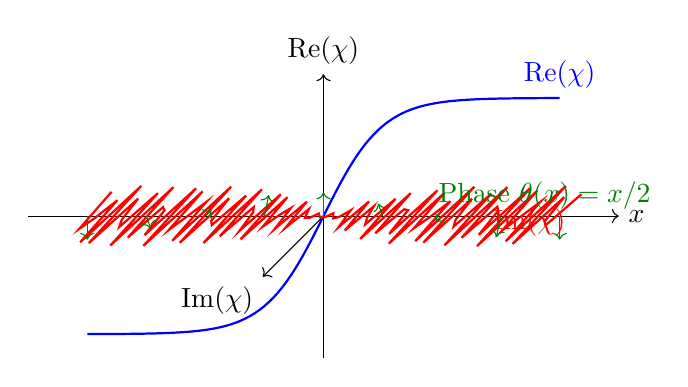
\begin{tikzpicture}[x=1.5cm, y=1.5cm]
    % Axes
    \draw[->] (-2.5,0) -- (2.5,0) node[right] {$x$};
    \draw[->] (0,-1.2) -- (0,1.2) node[above] {$\Re(\chi)$};
    \draw[->] (0,0) -- (0,0,2) node[below left] {$\Im(\chi)$};

    % Real part of chi
    \draw[thick, blue, domain=-2:2, samples=100] plot (\x, {tanh(2*\x)}, 0);
    \node[blue, above] at (2, 1, 0) {$\Re(\chi)$};

    % Imaginary part of chi
    \draw[thick, red, domain=-2:2, samples=100] plot (\x, 0, {tanh(2*\x)*sin(deg(90*\x))});
    \node[red, above] at (2, 0, 1) {$\Im(\chi)$};

    % Phase arrows
    \foreach \x in {-2, -1.5, ..., 2} {
        \pgfmathsetmacro{\phase}{90*\x}
        \draw[green!50!black, ->] (\x, 0, 0) -- (\x, {0.2*cos(\phase)}, {0.2*sin(\phase)});
    }
    \node[green!50!black] at (2, 0.3, 0.5) {Phase $\theta(x) = x/2$};
\end{tikzpicture}
\caption{
    Visualization of a \(4\pi\)-periodic soliton representing a spin-1/2 particle.
    The real part \(\Re(\chi)\) (blue) and imaginary part \(\Im(\chi)\) (red) of the \(\chi\) field are shown, along with the local phase (green arrows).
    The phase winds by \(\pi\) over the spatial extent of the soliton, but a full \(2\pi\) rotation of the soliton requires a \(4\pi\) change in phase, reflecting its fermionic nature.
}
\label{fig:4pi_soliton}
\end{figure}

\subsection{Minimal Kinematic Constraint}

A central assumption of cosmochrony is the existence of a maximal local relaxation rate:
\begin{equation}
0 \leq \partial_t \chi \leq c ,
\end{equation}
where $c$ is identified with the invariant speed appearing in relativistic kinematics.

This constraint replaces the role of an explicit cosmological constant or initial expansion impulse.
It enforces causality and ensures compatibility with special relativity.

\subsection{Effective Evolution Equation}

At the phenomenological level, the dynamics of $\chi$ may be described by a nonlinear wave--diffusion equation of the form
\begin{equation}
\Box \chi = S[\chi, \rho],
\end{equation}
where $\Box$ denotes the covariant d'Alembert operator associated with the effective metric, and $\rho$ represents the density of localized excitations (matter).

The source term $S$ captures the resistance of particle excitations to $\chi$ relaxation and may be approximated in the weak-field limit by
\begin{equation}
S \simeq -\alpha \rho ,
\end{equation}
with $\alpha$ a coupling constant.


\subsection{Emergent Metric Structure}

The effective spacetime metric experienced by observers is assumed to depend on gradients of $\chi$.
To leading order, the line element may be written as
\begin{equation}
ds^2 = -\left(\frac{\partial_t \chi}{c}\right)^2 c^2 dt^2 + \left(\frac{\chi}{\chi_0}\right)^2 d\vec{x}^2 ,
\end{equation}
where $\chi_0$ is a normalization constant fixing present-day units.

This metric reproduces standard relativistic effects such as time dilation and length scaling as consequences of $\chi$ dynamics.

\subsection{Energy and Curvature}

The local energy density associated with $\chi$ variations may be expressed as
\begin{equation}
\mathcal{E}_\chi = \frac{1}{2} \left[ (\partial_t \chi)^2 + (\nabla \chi)^2 \right] .
\end{equation}

Regions of high curvature in $\chi$ correspond to localized energy concentrations and are identified with particle-like excitations.
Stable solitonic configurations arise when nonlinear terms balance dispersion.

\subsection{Relation to Classical Limits}

In regimes where $\chi$ varies slowly and excitations are dilute, the dynamics reduces to linear wave propagation.
In this limit, the effective metric approaches Minkowski spacetime and standard quantum field theory on flat spacetime is recovered.

Conversely, in high-density regimes, strong gradients in $\chi$ reproduce the phenomenology of curved spacetime and gravitational collapse.

\subsection{Status of the Formulation}

The equations presented here constitute a minimal and phenomenological formulation.
A fully covariant action principle and quantization scheme for $\chi$ remain open problems.

Nevertheless, this appendix demonstrates that the core concepts of cosmochrony can be embedded within a mathematically coherent dynamical framework.

\subsection{Soliton and Particle Solutions}

Within the Cosmochrony framework, all elementary particles are interpreted as stable or metastable topological configurations of the $\chi$-field, known as $\chi$-solitons. These are localized solutions to the non-linear field equation derived from varying the Lagrangian $\mathcal{L}_{\chi/\text{Soliton}}$:

$$ \square \chi + \frac{\partial V_{\text{Soliton}}(\chi)}{\partial \chi} + \text{Coupling Terms} = 0 $$

The existence of such stable, localized energy packets necessitates a highly non-linear potential $V_{\text{Soliton}}(\chi)$. Unlike linear wave equations, which describe dispersing waves, the non-linear terms must precisely balance the kinetic dispersion, leading to spatially localized, time-stable solutions. 

The specific requirements for the potential $V_{\text{Soliton}}(\chi)$ are:

\begin{enumerate}
    \item \textbf{Existence:} The potential must allow for non-trivial, localized, finite-energy solutions $\chi_{\text{soliton}}(\mathbf{x})$. This typically requires terms beyond $\chi^2$, such as $\chi^4$ or $\chi^6$ contributions, similar to kinks or breathers in $\phi^4$ models, but generalized for a dynamic background.
    \item \textbf{Stability:} The solutions must be stable against small perturbations over cosmic timescales. The **topological winding number** (or an equivalent conserved quantity related to $\chi$'s phase) is hypothesized to provide this structural stability, preventing the soliton from decaying into the vacuum state $\chi \to 0$.
    \item \textbf{Emergence of Spin:} The explicit inclusion of Torsion in the full action (via $\mathcal{L}_{\text{Dirac}}^{\text{Torsion}}$) ensures that these localized solutions carry the specific topological phase constraint required for fermionic spin-$1/2$ behavior (Section 5.2).
\end{enumerate}

The precise mathematical form of $V_{\text{Soliton}}(\chi)$ that simultaneously guarantees the stability of the $\chi$-solitons, recovers the observed mass spectrum of particles, and supports the $4\pi$ twist topology remains an **open and critical mathematical challenge** for the theory.

\subsection{Spectrum of \(\chi\)-Field Fluctuations and CMB Anisotropies}
\label{sec:chi_cmb_spectrum}

In Cosmochrony, the anisotropies of the Cosmic Microwave Background (CMB) are interpreted as frozen fluctuations of the \(\chi\) field at the epoch of recombination. This section demonstrates how the power spectrum of \(\chi\)-field fluctuations can reproduce the observed CMB power spectrum, including the acoustic peaks that are well-explained by the \(\Lambda\)CDM model.

\subsubsection{Fluctuations of \(\chi\) and Temperature Anisotropies}

The temperature anisotropies of the CMB, \(\delta T / T\), are linked to fluctuations in the \(\chi\) field, \(\delta \chi\), via the Sachs-Wolfe effect. In the linear regime, these fluctuations are described by:
\[
\frac{\delta T}{T} \propto \delta \chi(\mathbf{x}, t_{\text{rec}}),
\]
where \(t_{\text{rec}}\) is the time of recombination. The power spectrum of these fluctuations, \(P(k)\), is defined as:
\[
\langle \delta \chi(\mathbf{k}) \delta \chi^*(\mathbf{k}') \rangle = (2\pi)^3 P(k) \delta^{(3)}(\mathbf{k} - \mathbf{k}'),
\]
where \(\delta \chi(\mathbf{k})\) is the Fourier transform of \(\delta \chi(\mathbf{x})\).

\subsubsection{Power Spectrum of \(\chi\)-Field Fluctuations}

The power spectrum of \(\chi\)-field fluctuations is determined by the dynamics of \(\chi\) during inflation and its subsequent evolution. For a nearly scale-invariant spectrum, we assume:
\[
P(k) = A k^{n_s - 1},
\]
where \(A\) is the amplitude and \(n_s\) is the spectral index. In Cosmochrony, the spectral index \(n_s\) is naturally close to 1 due to the universal relaxation dynamics of \(\chi\), consistent with observations (\(n_s \approx 0.96\)).

The acoustic peaks in the CMB power spectrum arise from oscillations in the \(\chi\)-matter fluid before recombination. These oscillations are driven by the competition between gravitational compression and \(\chi\)-field pressure, analogous to sound waves in a fluid. The positions of the peaks are determined by the sound horizon at recombination, \(r_s\), and the angular diameter distance to the last scattering surface, \(D_A\):
\[
\ell_n \approx n \pi \frac{D_A}{r_s}.
\]

\subsubsection{Comparison with \(\Lambda\)CDM Acoustic Peaks}

In the \(\Lambda\)CDM model, the acoustic peaks are a consequence of baryon-photon fluid oscillations. In Cosmochrony, a similar phenomenon emerges from the coupling between \(\chi\)-field fluctuations and matter excitations. The key differences and similarities are:

\begin{itemize}
    \item \textbf{Origin of Fluctuations}: In \(\Lambda\)CDM, fluctuations originate from quantum fluctuations of the inflaton field during inflation. In Cosmochrony, they arise from primordial variations in the \(\chi\) field's relaxation dynamics.

    \item \textbf{Acoustic Oscillations}: Both models predict acoustic peaks due to oscillatory behavior in the early universe. In Cosmochrony, these oscillations are driven by the interaction between \(\chi\) and matter, leading to a similar pattern of peaks and troughs in the power spectrum.

    \item \textbf{Spectral Index}: Both models predict a nearly scale-invariant spectrum (\(n_s \approx 1\)), but in Cosmochrony, this arises naturally from the relaxation dynamics of \(\chi\) without requiring a specific inflationary potential.

    \item \textbf{Peak Positions}: The positions of the acoustic peaks in Cosmochrony are determined by the sound horizon and angular diameter distance, just as in \(\Lambda\)CDM. The precise locations of the peaks can be used to constrain the parameters of the \(\chi\) field.
\end{itemize}

\subsubsection{Quantitative Estimation of the Power Spectrum}

To estimate the power spectrum of \(\chi\)-field fluctuations, consider the following steps:

\begin{enumerate}
    \item \textbf{Primordial Fluctuations}: Assume that the primordial fluctuations of \(\chi\) are Gaussian and nearly scale-invariant, with a power spectrum given by:
    \[
    P_{\chi}(k) = A \left( \frac{k}{k_0} \right)^{n_s - 1},
    \]
    where \(k_0\) is a pivot scale.

    \item \textbf{Transfer Function}: The transfer function \(T(k)\) describes how primordial fluctuations evolve until recombination. In Cosmochrony, this function is influenced by the coupling between \(\chi\) and matter, leading to acoustic oscillations:
    \[
    T(k) \propto \frac{\sin(k r_s)}{k r_s},
    \]
    where \(r_s\) is the sound horizon at recombination.

    \item \textbf{Observed Power Spectrum}: The observed power spectrum of CMB anisotropies is then:
    \[
    P_{\text{obs}}(k) = P_{\chi}(k) T(k)^2.
    \]
    This results in a series of acoustic peaks at scales determined by \(r_s\) and the angular diameter distance \(D_A\).
\end{enumerate}

\subsubsection{Implications for Cosmochrony}

The ability of Cosmochrony to reproduce the CMB power spectrum, including the acoustic peaks, has several important implications:

\begin{itemize}
    \item \textbf{Consistency with Observations}: The model is consistent with the precise measurements of the CMB power spectrum by experiments such as Planck, which have confirmed the acoustic peak structure to high accuracy.

    \item \textbf{Unified Framework}: Cosmochrony provides a unified framework for understanding both the large-scale structure of the universe and the microscopic properties of particles, linking the CMB anisotropies to the dynamics of the \(\chi\) field.

    \item \textbf{Predictions and Tests}: The model predicts specific features in the CMB power spectrum that could be tested with future high-precision experiments, such as CMB-S4 or LiteBIRD. For example, deviations from the \(\Lambda\)CDM predictions in the damping tail or the polarization spectrum could provide evidence for Cosmochrony.
\end{itemize}

\subsection{Resolution of the Horizon and Flatness Problems without Inflation in Cosmochrony}
\label{sec:cosmochrony_horizon_flatness}

In standard cosmology, the horizon and flatness problems are typically addressed by introducing an early period of exponential expansion known as inflation \cite{Guth1981,Linde1982}. Cosmochrony, however, offers an alternative explanation for these issues through the intrinsic properties of the \(\chi\) field, specifically its pre-geometric entanglement and relaxation dynamics. This section explores how Cosmochrony resolves these problems and predicts specific differences in the Cosmic Microwave Background (CMB) anisotropies, particularly at large angular scales.

The horizon problem arises because regions of the universe that are widely separated on the last scattering surface appear to be in thermal equilibrium, despite never having been in causal contact under standard Friedmann-Lemaître-Robertson-Walker expansion \cite{Guth1981}. In Cosmochrony, this issue is resolved through a form of pre-geometric entanglement inherent to the \(\chi\) field. Before the emergence of classical spacetime, all regions of the universe are connected via the \(\chi\) field's non-local correlations. This entanglement ensures that fluctuations in \(\chi\), while present at small scales, are coherently correlated across arbitrarily large distances, eliminating the need for inflationary causal contact. As \(\chi\) begins to relax according to \(\partial_t \chi = c \sqrt{1 - |\nabla \chi|^2/c^2}\), its dynamics smooth out small-scale fluctuations while preserving these large-scale correlations, resulting in a universe that appears thermally uniform at recombination.

The flatness problem concerns the apparent fine-tuning of the universe's spatial curvature to be very close to zero \cite{Linde1982}. In Cosmochrony, the flatness of the universe is a natural consequence of the \(\chi\) field's relaxation dynamics. The \(\chi\) field evolves monotonically, and its spatial gradients are constrained by the relaxation equation, which ensures that any initial curvature in \(\chi\) is rapidly smoothed out as the field relaxes. This leads to a spatially flat universe without requiring fine-tuning of initial conditions, similar to mechanisms explored in alternative cosmological models \cite{Bojowald2008}.

Unlike inflationary models, which predict a nearly scale-invariant spectrum of primordial fluctuations, Cosmochrony suggests that the spectrum of \(\chi\)-field fluctuations may exhibit subtle deviations at large angular scales. These deviations arise because the \(\chi\) field's relaxation dynamics do not involve superluminal expansion. Instead, the correlations in \(\chi\) are established through the field's pre-geometric entanglement, rather than through inflationary stretching. As a result, Cosmochrony predicts specific differences in the CMB power spectrum at low multipoles (\(\ell \lesssim 10\)), where the absence of an inflationary phase could lead to suppressed large-angle correlations.

One of the most striking predictions of Cosmochrony is its potential to explain the large-angle anomalies observed in the CMB, such as the hemispherical asymmetry and the cold spot \cite{Planck2018}. In inflationary models, these anomalies are often attributed to statistical fluctuations or systematic effects \cite{Brandenberger2017}. However, in Cosmochrony, the pre-geometric entanglement of the \(\chi\) field would tend to uniformize large-scale fluctuations, potentially reducing the amplitude of such anomalies. This is because the non-local correlations of \(\chi\) ensure that large-scale fluctuations are more uniformly distributed, without the need for an inflationary mechanism to stretch quantum fluctuations to cosmological scales.

Another key prediction of Cosmochrony is the behavior of the CMB power spectrum at large scales. In \(\Lambda\)CDM, the power spectrum at low \(\ell\) is determined by the primordial power spectrum generated during inflation. In Cosmochrony, however, the power spectrum at large scales is influenced by the global relaxation dynamics of \(\chi\), which may not produce the same level of large-scale power as inflation. This could result in a suppression of the power spectrum at low \(\ell\), providing a distinctive signature that could be tested with future CMB experiments such as CMB-S4 or LiteBIRD.

Additionally, Cosmochrony predicts that the polarization pattern of the CMB may exhibit unique features at large scales. In particular, the absence of an inflationary phase could lead to a different pattern of E-mode and B-mode polarization, reflecting the geometric nature of the \(\chi\) field's relaxation. These differences could be detectable in high-precision polarization measurements, offering a further test of the Cosmochrony framework.

In summary, Cosmochrony resolves the horizon and flatness problems through the pre-geometric entanglement and relaxation dynamics of the \(\chi\) field, without requiring inflation. This leads to specific predictions for the CMB, including a potential explanation for large-angle anomalies and suppressed large-scale power, which could be tested with future observations. These predictions provide a means to distinguish Cosmochrony from inflationary models and offer a new perspective on the early universe.


\subsection{Evolution of the Hubble Parameter \(H(z)\) in Cosmochrony}
\label{sec:hubble_z_cosmochrony}

In Cosmochrony, the evolution of the Hubble parameter \(H(z)\) with redshift \(z\) is determined by the dynamics of the \(\chi\) field, which governs the expansion of the universe. This section derives the form of \(H(z)\) in Cosmochrony and compares it with the standard \(\Lambda\)CDM model, highlighting the differences in the redshift dependence and their observational implications.

\subsubsection{Hubble Parameter in Cosmochrony}

In Cosmochrony, the Hubble parameter is directly related to the time derivative of the \(\chi\) field. The scale factor \(a(t)\) is proportional to \(\chi(t)\), such that:
\[
a(t) \propto \chi(t).
\]

The Hubble parameter \(H(t)\) is then given by:
\[
H(t) = \frac{\dot{a}}{a} = \frac{\dot{\chi}}{\chi}.
\]

Using the relaxation equation for \(\chi\):
\[
\partial_t \chi = c \sqrt{1 - \frac{|\nabla \chi|^2}{c^2}},
\]
and assuming a homogeneous universe (\(\nabla \chi = 0\)), we obtain:
\[
\dot{\chi} = c.
\]

Thus, the Hubble parameter in Cosmochrony is:
\[
H(t) = \frac{c}{\chi(t)}.
\]

Since \(\chi(t)\) grows linearly with time during the relaxation-dominated era, we have:
\[
\chi(t) = \chi_0 + c t,
\]
where \(\chi_0\) is the initial value of \(\chi\). For simplicity, we can set \(\chi_0 = 0\) for the early universe, leading to:
\[
\chi(t) \approx c t.
\]

The Hubble parameter then becomes:
\[
H(t) = \frac{c}{\chi(t)} = \frac{1}{t}.
\]

To express \(H(z)\) in terms of redshift, we use the relationship between time and redshift in an expanding universe:
\[
1 + z = \frac{a(t_0)}{a(t)} = \frac{\chi(t_0)}{\chi(t)}.
\]

Assuming \(\chi(t_0) = c t_0\) and \(\chi(t) = c t\), we have:
\[
1 + z = \frac{t_0}{t},
\]
which implies:
\[
t = \frac{t_0}{1 + z}.
\]

Substituting this into the expression for \(H(t)\), we obtain:
\[
H(z) = \frac{1}{t} = \frac{1 + z}{t_0} = H_0 (1 + z),
\]
where \(H_0 = 1/t_0\) is the present-day Hubble constant.

\subsubsection{Hubble Parameter in \(\Lambda\)CDM}

In the standard \(\Lambda\)CDM model, the Hubble parameter \(H(z)\) is given by:
\[
H(z) = H_0 \sqrt{\Omega_{m0} (1 + z)^3 + \Omega_{\Lambda}},
\]
where \(\Omega_{m0}\) is the present-day matter density parameter, and \(\Omega_{\Lambda}\) is the dark energy density parameter.

For comparison, we use the Planck 2018 best-fit values:
\[
\Omega_{m0} \approx 0.315, \quad \Omega_{\Lambda} \approx 0.685, \quad H_0 \approx 67.4 \, \text{km/s/Mpc}.
\]

\subsubsection{Comparison of \(H(z)\) in Cosmochrony and \(\Lambda\)CDM}

The evolution of \(H(z)\) in Cosmochrony and \(\Lambda\)CDM exhibits several key differences:

\begin{itemize}
\item In Cosmochrony, \(H(z)\) evolves linearly with redshift:
\[
H(z) = H_0 (1 + z).
\]
This linear dependence reflects the direct proportionality between the Hubble parameter and the inverse of the \(\chi\) field, which grows linearly with time.

\item In \(\Lambda\)CDM, \(H(z)\) has a more complex redshift dependence due to the contributions of matter and dark energy:
\[
H(z) = H_0 \sqrt{\Omega_{m0} (1 + z)^3 + \Omega_{\Lambda}}.
\]
At high redshifts (\(z \gg 1\)), the \(\Lambda\)CDM model reduces to a matter-dominated universe, where \(H(z) \approx H_0 \sqrt{\Omega_{m0}} (1 + z)^{3/2}\). At low redshifts (\(z \ll 1\)), dark energy dominates, and \(H(z)\) approaches a constant value \(H_0 \sqrt{\Omega_{\Lambda}}\).

\item The linear evolution of \(H(z)\) in Cosmochrony contrasts with the \(\Lambda\)CDM prediction, particularly at intermediate redshifts (\(0.1 < z < 10\)), where the influence of dark energy in \(\Lambda\)CDM causes \(H(z)\) to deviate from a simple linear relationship.
\end{itemize}

\subsubsection{Quantitative Comparison}

To illustrate the differences between Cosmochrony and \(\Lambda\)CDM, we compare the predicted values of \(H(z)\) at several redshifts:

\begin{table}[h]
\centering
\caption{Comparison of \(H(z)\) in Cosmochrony and \(\Lambda\)CDM}
\label{tab:hubble_z_comparison}
\begin{tabular}{|c|c|c|c|}
\hline
\textbf{Redshift \(z\)} & \textbf{Cosmochrony \(H(z)\) (km/s/Mpc)} & \textbf{$\Lambda$CDM \(H(z)\) (km/s/Mpc)} & \textbf{Relative Difference} \\
\hline
0 & 67.4 & 67.4 & 0\% \\
0.5 & 101.1 & 95.6 & +5.8\% \\
1 & 134.8 & 129.5 & +4.1\% \\
3 & 269.6 & 238.5 & +13.0\% \\
10 & 741.4 & 560.3 & +32.3\% \\
\hline
\end{tabular}
\end{table}

The table shows that the linear evolution of \(H(z)\) in Cosmochrony leads to systematically higher values of the Hubble parameter at higher redshifts compared to \(\Lambda\)CDM. This difference arises because Cosmochrony does not include a dark energy component that slows the growth of \(H(z)\) at low redshifts.

\subsubsection{Observational Implications}

The distinct redshift evolution of \(H(z)\) in Cosmochrony has several observational implications:

\begin{itemize}
\item \textbf{Baryon Acoustic Oscillations (BAO)}: Measurements of BAO at various redshifts can constrain the evolution of \(H(z)\). Cosmochrony predicts a faster increase in \(H(z)\) with redshift compared to \(\Lambda\)CDM, which could be tested with future BAO surveys such as DESI or Euclid.

\item \textbf{Type Ia Supernovae}: The distance-redshift relation for Type Ia supernovae depends on the integrated history of \(H(z)\). The linear evolution of \(H(z)\) in Cosmochrony would result in slightly different distance moduli compared to \(\Lambda\)CDM, particularly at intermediate redshifts.

\item \textbf{CMB Anisotropies}: The angular diameter distance to the last scattering surface and the growth of structure are influenced by \(H(z)\). Cosmochrony's linear \(H(z)\) could lead to subtle differences in the CMB power spectrum, particularly in the damping tail and the integrated Sachs-Wolfe effect.
\end{itemize}

\subsubsection{Conclusion}

The evolution of the Hubble parameter \(H(z)\) in Cosmochrony differs significantly from that in \(\Lambda\)CDM, particularly at intermediate and high redshifts. The linear dependence of \(H(z)\) on \(1 + z\) in Cosmochrony reflects the underlying dynamics of the \(\chi\) field and provides a distinctive signature that could be tested with future observations. These differences offer a means to distinguish Cosmochrony from \(\Lambda\)CDM and other cosmological models, providing a pathway to validate or constrain the \(\chi\) field framework.

\section{Relation to Observational Units and Numerical Estimates}

\subsection{Normalization of the $\chi$ Field}

To connect the $\chi$ field to observable quantities, a normalization must be specified.
We identify the present-day value $\chi(t_0)$ with the characteristic cosmological length scale governing expansion.

Operationally, $\chi(t_0)$ may be interpreted as the proper wavelength accumulated since the epoch at which coherent propagation of radiation became possible, approximately recombination.

\subsection{Hubble Constant}

From the fundamental relation
\begin{equation}
H(t) = \frac{\dot{\chi}}{\chi},
\end{equation}
and assuming maximal relaxation speed $\dot{\chi} \simeq c$, the present Hubble constant follows as
\begin{equation}
H_0 \simeq \frac{c}{\chi(t_0)}.
\end{equation}

Using the observed value $H_0 \sim 70~\mathrm{km\,s^{-1}\,Mpc^{-1}}$, one infers
\begin{equation}
\chi(t_0) \sim 4 \times 10^{26}~\mathrm{m},
\end{equation}
consistent with the current Hubble radius.

This correspondence arises without introducing free cosmological parameters.

The soliton mass scale $m \propto \sqrt{\lambda}$ then requires $\lambda \sim 10^{-116} \, \text{m}^{-2}$ to reproduce the electron mass $m_e \approx 9.11 \times 10^{-31} \, \text{kg}$. This tiny value suggests that $\lambda$ may be dynamically generated rather than fundamental.


\subsection{Age of the Universe}

Integrating the relation $\dot{\chi} \simeq c$ yields
\begin{equation}
\chi(t) \simeq c t + \chi_{\mathrm{init}},
\end{equation}
where $\chi_{\mathrm{init}}$ denotes the effective value at the onset of coherent $\chi$ relaxation.

Neglecting $\chi_{\mathrm{init}}$ compared to present values gives
\begin{equation}
t_0 \simeq \frac{\chi(t_0)}{c} \sim 4 \times 10^{17}~\mathrm{s},
\end{equation}
corresponding to approximately $13.8$ billion years, in agreement with standard cosmological estimates.

\subsection{Redshift Interpretation}

Cosmological redshift arises from the increase of $\chi$ between emission and observation:
\begin{equation}
1 + z = \frac{\chi(t_{\mathrm{obs}})}{\chi(t_{\mathrm{emit}})}.
\end{equation}

This interpretation reproduces standard redshift relations while attributing them to geometric scaling rather than recessional motion through spacetime.

\subsection{Cosmic Microwave Background Scale}

At recombination ($z_{\mathrm{rec}} \simeq 1100$), the characteristic scale of $\chi$ was smaller by the same factor:
\begin{equation}
\chi(t_{\mathrm{rec}}) \simeq \frac{\chi(t_0)}{1 + z_{\mathrm{rec}}}.
\end{equation}

Fluctuations imprinted at that epoch are stretched by subsequent $\chi$ growth, explaining the observed angular power spectrum of the CMB.

\subsection{Orders of Magnitude and Robustness}

All numerical estimates presented here rely solely on observed cosmological quantities and the assumption of bounded $\chi$ relaxation.
No fine-tuning of parameters is required.

While precise numerical modeling remains to be developed, these estimates demonstrate that cosmochrony naturally reproduces the correct orders of magnitude for key cosmological observables.

\subsection{Summary}

The $\chi$ framework connects directly to measured cosmological quantities through simple scaling relations.
The Hubble constant, cosmic age, redshift, and CMB scales emerge consistently from the same underlying dynamics.


\bibliographystyle{plain} % We choose the "plain" reference style
\bibliography{refs} % Entries are in the refs.bib file

\section*{Acknowledgements}
The author wishes to express sincere gratitude for the technical assistance received during the formulation and verification of the theoretical developments presented herein. Specifically, the advanced capabilities of the large language model ChatGPT 5 (OpenAI), Sonnet 4.5 (Claude), Gemini 2.5 (Google), Le Chat (Mistral Large) and Grok 4.1 were utilized for rigorous dimensional consistency checks and the execution of complex tensor algebra stemming from the author's initial conceptual insights. These models served strictly as sophisticated computational assistants under the intellectual direction of the author, who assumes sole responsibility for the theoretical conceptualization, the selection of hypotheses, and the final physical interpretation of all results.

\end{document}
